\documentclass[fleqn]{NotesClass}

\usepackage{subcaption}
\usepackage{mathtools}
\usepackage{csquotes}
\usepackage{tikz-cd}
\usepackage{enumitem}
\usepackage{colortbl}
\usepackage[polutonikogreek, english]{babel}
\usepackage{multicol}
\usepackage{siunitx}
\usepackage[version=4]{mhchem}
\usepackage{chemfig}

% Tikz stuff
\usepackage{tikz}
\tikzset{>=latex}
% external
\usetikzlibrary{external}
\tikzexternalize[prefix=tikz-external/]
%\tikzexternaldisable
% other libraries

% References, should be last things loaded
\usepackage{hyperref}  % Should be loaded second last (cleveref last)
\colorlet{hyperrefcolor}{blue!60!black}
\hypersetup{colorlinks=true, linkcolor=hyperrefcolor, urlcolor=hyperrefcolor}
\usepackage[
capitalize,
nameinlink,
noabbrev
]{cleveref} % Should be loaded last

% My packages
\usepackage{NotesBoxes}
\usepackage{NotesMaths}

% Title page info
\title{Symmetries of Quantum Mechanics}
\author{Willoughby Seago}
\date{}
% \subtitle{}
% \subsubtitle{}

% Highlight colour
\definecolor{highlight}{HTML}{710D78}
\definecolor{my blue}{HTML}{2A0D77}
\definecolor{my red}{HTML}{770D38}
\definecolor{my green}{HTML}{14770D}

% Commands
% Maths
\NewDocumentCommand{\presentation}{ s o m m }{
    \IfNoValueTF{#2}{
        \IfBooleanTF{#1}{
            \left\langle #3 \, \middle\vert \, #4 \right\rangle
        }{
            \langle #3 \, \vert \, #4 \rangle
        }
    }{
        #2\langle #3 \, #2\vert \, #4 #2\rangle
    }
}
\DeclarePairedDelimiterX{\groupindex}[2]{[}{]}{#1 : #2}
\newcommand*{\union}{\cup}
\newcommand*{\bigunion}{\bigcup}
\newcommand*{\intersection}{\cap}
\newcommand*{\bigintersection}{\bigcap}
\newcommand{\subgroup}{\subset}
\newcommand{\subgroupeq}{\subseteq}
\newcommand{\supgroup}{\supset}
\newcommand{\supgroupeq}{\supseteq}
\renewcommand{\emptyset}{\emptysetAlt}
\newcommand*{\action}{\mathbin{.}}
\newcommand*{\isomorphic}{\cong}
\DeclareMathOperator{\image}{Im}
\DeclarePairedDelimiterX{\innerprod}[2]{\langle}{\rangle}{#1, #2}
\newcommand*{\trans}{\top}
\newcommand*{\hermit}{\dagger}
\newcommand*{\positiveintegers}{\integers_{>0}}
\newcommand*{\hilbert}{\mathcal{H}}
\newcommand*{\ident}{\mathbf{1}}
\DeclareMathOperator{\tr}{tr}
\newcommand*{\directsum}{\oplus}
\newcommand*{\directproduct}{\otimes}
\DeclareMathOperator{\Hom}{Hom}
\newcommand*{\e}{\mathrm{e}}
\DeclareMathOperator{\isometry}{ISO}
\newcommand{\orbit}{\mathit{g}}
\DeclareMathOperator{\Aut}{Aut}
\newcommand*{\normalsubgroup}{\vartriangleleft}
\newcommand*{\normalsubgroupeq}{\trianglelefteq}
\newcommand*{\longsim}{\scalebox{2.5}[1.1]{\(\sim\)}}
\DeclareMathOperator{\ISO}{ISO}
\newcommand{\triangleDthree}[3]{%
    \begin{tikzpicture}[baseline=(current bounding box), scale=0.5, font=\tiny]
        \draw[highlight, very thick, rounded corners=0.1, fill=highlight!20] (-30:1) -- (90:1) -- (210:1) -- cycle;
        \node at (210:1.3) {#1};
        \node at (90:1.3) {#2};
        \node at (-30:1.3) {#3};
    \end{tikzpicture}%
}

% Include
\includeonly{parts/math-prelim-appendix, parts/groups-appendix}

\begin{document}
    \frontmatter
    \titlepage
    \innertitlepage{tikz-external/ethane} 
    \tableofcontents
    \mainmatter
    \chapter{Introduction}
    \section{Binary Operations}
    
    \begin{dfn}{Binary Operation}{}
        A \define{binary operation}\index{binary!operation} on a set \(X\) is a map, \(f\colon X \times X \to X\).
        
        \begin{rmk}
            We say that \(X\) is \defineindex{closed} under the binary operation since combining two elements of \(X\) gives another element of \(X\).
        \end{rmk}
    \end{dfn}
    
    \begin{ntn}{}{}
        Binary operations are usually written with infix notation, for example, the binary operation \(\cdot \colon X \times X \to X\) maps \((x, x') \mapsto x \cdot x'\) whereas for a normal function, say, \(f\colon X \times X \to X\), we usually use prefix notation: \((x, x') \mapsto f(x, x')\).
        
        The other common notation when there is only one (obvious) choice of binary operation is juxtaposing the two elements, for example \((x, x') \mapsto xx'\).
        This is exactly what we do with multiplication most of the time rather than writing \(x \cdot x\), or, \(x \times x\).
        We will use this notation most of the time, particularly when the binary operation is denoted \(\cdot\), and we will not comment on it further.
    \end{ntn}
    
    The notion of a binary operation is very general.
    We typically restrict ourselves to various classes of binary operations which are easier to work with due to possessing various properties.
    
    \subsection{Associativity}
    \begin{dfn}{Associativity}{}
        We say that the binary operation \(\cdot\colon X \times X \to X\) is \defineindex{associative} if
        \begin{equation}
            x \cdot (y \cdot z) = (x \cdot y) \cdot z.
        \end{equation}
    \end{dfn}
    
    From this it follows that an associative binary operation and any number of elements in a product the answer will be the same no matter how we write the brackets and so we usually don't write any brackets at all.
    For example, with four elements two possible ways to write the product of four elements are
    \begin{equation}
        (x_1 x_2) (x_3 x_4) = x_1(x_2(x_3x_4)) = x_1 x_2 x_3 x_4.
    \end{equation}
    Writing \(x_3x_4 = x\) it follows that \((x_1x_2)(x_3x_4) = (x_1x_2)x = x_1(x_2x) = x_1(x_2(x_3x_4))\) where the second equality is where we apply the associativity axiom.
    
    \begin{exm}{Function Composition}{}
        Denote by \(\Hom(A, B)\) the set of functions from \(A\) to \(B\).
        We define \defineindex{function composition} to be the binary operation \(\circ\colon \Hom(B, C) \times \Hom(A, B) \to \Hom(A, C)\) for sets \(A\), \(B\), and \(C\), such that for \(f \in \Hom(B, C)\) and \(g \in \Hom(A, B)\) we have
        \begin{equation}
            (f \circ g)(a) = f(g(a))
        \end{equation}
        for all \(a \in A\).
        An alternative way of saying this is that the following diagram commutes, meaning that the result is independent of the path taken:
        \begin{equation}
            \tikzexternaldisable
            \begin{tikzcd}[row sep=1.5cm, column sep=1.5cm]
                A \ar[r, "g"] \ar[dr, "f \circ g", swap] & B \ar[d, "f"] \\
                & C.
            \end{tikzcd}
            \tikzexternalenable
        \end{equation}
        
        Function composition is associative.
        That is if \(f \in \Hom(A, B)\), \(g \in \Hom(B, C)\), and \(h \in \Hom(C, D)\) then
        \begin{equation*}
            (f \circ (g \circ h))(d) = f((g\circ h)(d)) = f(g(h(d))) = (f\circ g)(h(d)) = ((f\circ g)\circ h)(d),
        \end{equation*}
        or in other words
        \begin{equation}
            f \circ (g \circ h) = (f \circ g) \circ h
        \end{equation}
        and so \(\circ\) is associative.
        
        The commutative diagram expressing this fact is
        \begin{equation}
            \tikzexternaldisable
            \begin{tikzcd}[column sep=1.5cm]
                A \ar[r, "f"] \ar[rr, "g \circ f", bend left] \ar[rrr, "h \circ g \circ f", bend right, swap] & B \ar[r, "g"] \ar[rr, "h \circ g", bend left] & C \ar[r, "h"] & D.
            \end{tikzcd}
            \tikzexternalenable
        \end{equation}
        
        One important corollary is that matrix multiplication is just composition of linear maps and so matrix multiplication is associative.
    \end{exm}
    
    Many of the binary operations that we are familiar with are associative, such as addition, and multiplication, but not all, for example, subtraction isn't associative, consider \(5 - (2 - 3) = 6\) and \((5 - 2) - 3 = 0\).
    
    \begin{exm}{Nonassociativity}{}
        An example of a binary operation that \emph{isn't} associative is the vector cross product, \(\times\colon\reals^3 \times \reals^3 \to \reals^3\) (note that the first \(\times\) is the cross product of vectors and the second one is the Cartesian product of sets).
        This can be shown by an example.
        Take \(\vv{a} = (1, 1, 0)^\trans\), \(\vv{b} = (0, 1, 0)^\trans\), and \(\vv{c} = (0, 0, 1)^\trans\).
        Then
        \begin{equation}
            \vv{a} \times \vv{b} = 
            \begin{pmatrix}
                0\\ 0\\ -1
            \end{pmatrix}
            \implies (\vv{a} \times \vv{b}) \times \vv{c} = 
            \begin{pmatrix}
                0\\ 0\\ -1
            \end{pmatrix}
        \end{equation}
        whereas
        \begin{equation}
            \vv{b} \times \vv{c} = 
            \begin{pmatrix}
                1\\ 0\\ 0
            \end{pmatrix}
            \implies \vv{a} \times (\vv{b} \times \vv{c}) = 
            \begin{pmatrix}
                0\\ 0\\ 0
            \end{pmatrix}
            .
        \end{equation}
    \end{exm}
    
    \subsection{Identity}
    \begin{dfn}{Identity}{}
        Given a set, \(X\), and a binary operation on \(X\), \(\cdot \colon X \times X \to X\), we say that \(e \in X\) is the \defineindex{identity} if
        \begin{equation}
            x \cdot e = e \cdot x = x
        \end{equation}
        for all \(x \in X\).
    \end{dfn}
    
    \begin{ntn}{Identities}{}
        There are many notations for identities since it is an idea that emerged in many different areas before being unified by group theory and other algebraic concepts.
        The notation we will choose typically depends on both what the elements of \(X\) are and the nature of \(\cdot\).
        For example,
        \begin{itemize}
            \item if the elements of \(X\) are matrices then the identity may be denoted \(I\), or \(\mathbb{1}\),
            \item if the elements of \(X\) are functions then the identity may be denoted \(\mathrm{id}\), or \(\iota\),
            \item if \(\cdot\) can be thought of as multiplication then the identity is often denoted \(1\), and
            \item if \(\cdot\) can be thought of as addition (in which case we are more likely to denote the operation \(+\)) then the identity is often denoted \(0\).
        \end{itemize}
    \end{ntn}
    
    \begin{exm}{Identities}{}
        \begin{itemize}
            \item The identity for multiplication in \(\reals\) is 1.
            \item The identity for addition in \(\rationals\) is 0.
            \item The identity for matrix multiplication is \(I\), which has \(\delta_{ij}\) as elements.
            \item The identity function is \(\mathrm{id}_X \colon X \times X \to X\) defined by \(\mathrm{id}_X(x) = x\) for all \(x \in X\).
        \end{itemize}
    \end{exm}
    
    Not all binary operations have an identity, for example, there is no identity for the cross product.
    It is also important that the identity must be an element of \(X\).
    For example if we set \(X = \positiveintegers\)\footnote{\(\positiveintegers \coloneqq \{1, \dotsc\} = \naturals \setminus \{0\}\)} and take our operation to be addition then there is no identity since \(0 \notin \positiveintegers\).
    
    \subsection{Inverse}
    \begin{dfn}{Inverse}{}
        Given a set, \(X\), and a binary operation on \(X\), \(\cdot \colon X \times X \to X\), such that \(e \in X\) acts as an identity element then we say that \(x \in X\) has an \defineindex{inverse} in \(X\) if there exists some \(x^{-1} \in X\) such that
        \begin{equation}
            x \cdot x^{-1} = x^{-1} \cdot x = e.
        \end{equation}
    \end{dfn}
    
    \begin{ntn}{Inverses}{}
        If we think of the binary operation, \(\cdot\), as multiplicative then we write the inverse of \(x\) as \(x^{-1}\), taking inspiration from division being the inverse of multiplication.
        
        If we think of the binary operation, \(+\), as additive then we write the inverse of \(x\) as \(-x\), and we write \(y - x\) as shorthand for \(y + (-x)\), taking inspiration from subtraction being the inverse of multiplication.
    \end{ntn}
    
    As with the identity it is important that the inverse is an element of \(X\).
    For example, taking \(X = \naturals\)\footnote{\(\naturals \coloneqq \{0, 1, \dotsc\} = \positiveintegers \union \{0\}\).} and our operation to be addition we have an identity, \(0 \in \naturals\), but no inverses (apart from 0, which is its own inverse), since, for example, \(-3\) is the inverse of \(3\), but \(-3 \notin \naturals\).
    
    \section{Groups}
    \begin{dfn}{Group}{dfn:group}
        Formally a \defineindex{group} is an ordered pair, \((G, \cdot)\), where \(G\) is a set and \(\cdot\) is a binary operation on \(G\) satisfying the following \defineindex{group axioms}:
        \begin{enumerate}
            \item \define{Associativity}: For all \(g_1, g_2, g_3 \in G\)
            \begin{equation}
                g_1 \cdot (g_2 \cdot g_3) = (g_1 \cdot g_2) \cdot g_3.
            \end{equation}
            \item \define{Identity}: There exists some \(e \in G\) such that \(e \cdot g = g \cdot e = g\).
            \item \define{Inverse}: For all \(g \in G\) there exists some \(g^{-1}\) such that
            \begin{equation}
                g\cdot g^{-1} = g^{-1} \cdot g = e
            \end{equation}
            where \(e\) is the identity of the group.
        \end{enumerate}
        \begin{rmk}
            In practice we don't really think of groups as an ordered pair, \((G, \cdot)\), but as a set and an operation on the set and rather than saying \enquote{the group \((G, \cdot)\)} most of the time we will say \enquote{the group \(G\) under \(\cdot\)}, or simply \enquote{the group \(G\)} when it is clear what the group operation.
        \end{rmk}
        
        Some sources include a fourth axiom:
        \begin{enumerate}[resume]
            \item \define{Closure}: The product of two elements of a group is another element of the group.
        \end{enumerate}
        This is implicit however in the definition of a binary operation as a function \(X \times X \to X\) and so we leave it out.
        It will be important to consider when we think about subgroups by restricting the binary operation to a subset.
    \end{dfn}
    
    \begin{ntn}{Multiple Groups}{}
        Say \(G\) and \(H\) are two groups of interest.
        Then we will use \(G\) and \(H\) as subscripts to differentiate between the two groups.
        For example the product of two elements in \(G\) may be written as \(g \cdot_G g'\), as opposed to \(g \cdot_H g'\), which is the product of \(H\) applied to elements of \(G\), as we may sometimes have reason to do if, say, \(H \subseteq G\).
        The identity in \(H\) may be denoted \(e_H\), and so \(e_H \cdot_H h = h\), but we may not have \(h \cdot_G e_H = h\), since a different operation means we can have a different identity.
    \end{ntn}
    
    \begin{lma}{}{}
        The identity of a group is unique.
        
        \begin{proof}
            Suppose that \(G\) is a group and \(e, e' \in G\) both act as identities.
            That is \(e'g = ge = g\) for all \(g \in G\).
            Then \(e = e'e = e'\) where the first equality holds by the identity property of \(e'\) and the second by the identity property of \(e\).
            This means \(e = e'\) and so the identity is unique.
        \end{proof}
    \end{lma}
    
    \begin{lma}{}{}
        The inverse of a group element is unique.
        
        \begin{proof}
            Suppose that \(G\) is a group and \(g \in G\) is such that \(h, h' \in G\) act as inverses to \(G\).
            That is \(hg = gh' = e\) where \(e \in G\) is the identity of \(G\).
            Right multiplying \(hg = gh' = e\) by \(h'\) we have \(hgh' = gh'h'\).
            Using the inverse property of \(h'\) on both sides we have \(he = eh'\) which implies \(h = h'\) and so the inverse is unique.
        \end{proof}
    \end{lma}
    
    \begin{lma}{}{lma:socks and shoes}
        Let \(G\) be a group and \(g, h \in G\).
        Then \((gh)^{-1} = h^{-1}g^{-1}\).
        \begin{proof}
            The defining property of the inverse is that \(gg^{-1} = e\) so we simply need to show that \((gh)(h^{-1}g^{-1}) = e\) and we can then identify that \(h^{-1}g^{-1} = (gh)^{-1}\).
            Using associativity we can rewrite the brackets in the expression however we like and so we have \((gh)(h^{-1}g^{-1}) = g(hh^{-1})g^{-1} = geg^{-1} = gg^{-1} = e\).
        \end{proof}
    \end{lma}
    
    \begin{lma}{}{lma:inverse cancels inverse}
        Let \(G\) be a group, and \(g \in G\).
        Then \((g^{-1})^{-1} = g\).
        \begin{proof}
            If \((g^{-1})^{-1} = g\) then we expect that \((g^{-1})^{-1}g^{-1} = e\).
            We can identify that \((g^{-1})^{-1}g^{-1} = (gg^{-1})^{-1}\) using \cref{lma:socks and shoes}.
            We then have \((g^{-1})^{-1}g^{-1} = (gg^{-1})^{-1} = e^{-1} = e\), since \(ee = e\), so clearly \(e^{-1} = e\).
        \end{proof}
    \end{lma}
    
    \subsection{Examples of Groups}
    \begin{exm}{Additive Groups}{}
        \(\integers\), \(\rationals\), \(\reals\), and \(\complex\) all form groups under addition.
        In particular the identity is \(0\), and the inverse of \(x\) is \(-x\).
    \end{exm}
    
    These same sets don't form groups under multiplication.
    The identity of multiplication is 1, and there is no number which acts as an inverse for multiplication by zero, that is there are no solutions to \(0x = 1\) in \(\integers\), \(\rationals\), \(\reals\), or \(\complex\).
    Noticing that zero causes issues with division it's sensible to consider these sets with zero removed.
    Denote by \(\integers^* \coloneqq \integers \setminus \{0\}\) the set of integers with zero removed.
    This is not a group since, for example, the multiplicative inverse of 2 is \(1/2\), and \(1/2 \notin \integers^*\).
    
    \begin{exm}{Multiplicative Groups}{}
        \(\rationals^*\), \(\reals^*\), and \(\complex^*\)\index{\(-^*\), nonzero elements} all form a group under multiplication, where we use the notation \(\rationals^* \coloneqq \rationals \setminus \{0\}\), \(\reals^* \coloneqq \reals \setminus \{0\}\), and \(\complex^* \coloneqq \complex \setminus \{0\}\).
        The identity is 1 and the inverse of \(x\) is \(1/x\).
    \end{exm}
    
    \begin{dfn}{Permutation}{}
        Formally a \defineindex{permutation} on \(n\) objects is a bijection
        \begin{equation}
            \sigma \colon \{1, \dotsc, n\} \to \{1, \dotsc, n\}.
        \end{equation}
        This idea can be extended to any set of size \(n\), not just \(\{1, \dotsc, n\}\).
        Informally we can think of a permutation as a way of ordering the \(n\) objects such that the \(m\)th object is in position \(\sigma(m)\).
    \end{dfn}
    
    \begin{exm}{Permutation Group}{}
        The \defineindex{permutation group}\index{Sn@\(S_n\), permutation group}, \(S_n\), defined as the set of all permutations on \(n\) objects, is a group under function composition.
        What this means is that if we permute the objects then permute them again we will have a permutation of the objects (closure), we can always leave the objects in the order they are (identity), and we can always undo a permutation (inverse).
    \end{exm}
    
    \begin{exm}{Cyclic Group}{}
        Take some \(n \in \positiveintegers\).
        We define \(\integers_n \coloneqq \{\e^{2i\pi m/n} \mid m = 0, \dotsc, n - 1\}\).
        This is a group under multiplication, called the \defineindex{cyclic group}\index{Zn@\(\integers_n\), cyclic group} of order \(n\).
        
        Instead define \(\integers_n \coloneqq \{0, \dotsc, n - 1\}\).
        This is a group under addition modulo \(n\).
        This is actually the same group as the previous definition of \(\integers_n\) (they are isomorphic, a term defined later in \cref{def:morphism}).
    \end{exm}
    
    \begin{exm}{Rotation Group}{}
        Define \(\orthogonal(3) \coloneqq \{ O \in \matrices{3}{\reals} \mid  O^\trans O = \ident\}\).
        This is a group under matrix multiplication.
        The identity is the identity matrix and the inverse is the normal matrix inverse, which is guaranteed to exist since for \(O \in \orthogonal(3)\) we have \(\det O = \pm 1 \ne 0\).
        This is called the \defineindex{rotation group}\index{O(3)@\(\orthogonal(3)\), rotation group}.
        
        \begin{rmk}
            Strictly this is the fundamental representation of \(\orthogonal(3)\).
        \end{rmk}
    \end{exm}
    
    \subsection{Basic Definitions}
    \begin{dfn}{Group Size}{}
        Given some group \(G\) we classify it as \defineindex{finite}, \defineindex{discrete}, or \defineindex{continuous}, depending on whether \(G\) has a finite number of elements, the same number of elements as \(\integers\), or more elements than \(\integers\).
    \end{dfn}
    
    Recall that two sets have the same cardinality if there is a bijection between them.
    For example, \(\integers\), \(\positiveintegers\), \(\naturals\), and \(\rationals\) all have the same cardinality.
    A set is larger than a second set if there is an injective function from the first set to the second, but not vice versa.
    For example, there are more real numbers than integers.
    
    \begin{exm}{}{}
        Of the groups mentioned so far \(S_n\), and \(\integers_n\) are finite.
        \(\integers\), \(\rationals\), \(\integers^*\), and \(\rationals^*\) are discrete.
        \(\reals\), \(\complex\), \(\reals^*\), \(\complex^*\), and \(\orthogonal(3)\) are continuous.
    \end{exm}
    
    \begin{dfn}{Order}{}
        The \define{order}\index{order!group} of a finite group, \(G\), is the number of elements in \(G\), denoted \(\abs{G}\).
        
        Given some group, \(G\), the \define{order}\index{order!element} of \(g \in G\) is the smallest \(n \in \positiveintegers\) such that \(g^n = e\), where \(e\) is the group identity and \(g^n\) has the expected meaning of the product of \(g\) with itself \(n\) times.
        
        Note that the order of the identity is always 1.
    \end{dfn}
    
    \begin{exm}{Order}{}
        The order of \(S_n\) is \(\abs{S_n} = n!\).
        The order of \(\integers_n\) is \(\abs{\integers_n} = n\).
        
        The order of \(\e^{2i\pi 3/9} = \e^{2i\pi/3} \in \integers_9\) is 3 since \((\e^{2i\pi/3})^1 = \e^{2i\pi/3}\), \((\e^{2i\pi/3})^2 = \e^{4i\pi/3}\), and \((\e^{2i\pi/3})^3 = \e^{6i\pi/3} = \e^{2i\pi} = 1\), which is the identity of \(\integers_n\).
    \end{exm}
    
    \begin{dfn}{Abelian}{}
        A group, \(G\), is \defineindex{Abelian} if all of its elements commute.
        That is \(gg' = g'g\) for all \(g \in G\).
        If this is not the case we say that \(G\) is non-Abelian.
    \end{dfn}
    
    \begin{exm}{Abelian}{}
        Of the groups mentioned so far \(\integers\), \(\rationals\), \(\reals\), \(\complex\), \(\rationals^*\), \(\reals^*\), \(\complex^*\), and \(\integers^*\) are Abelian.
        \(S_n\) and \(\orthogonal(3)\) are non-Abelian.
    \end{exm}
    
    \begin{dfn}{Subgroup}{}
        Let \(G\) be a group.
        We say that \(H\) is a \defineindex{subgroup} of \(G\), denoted \(H \subgroupeq G\), if
        \begin{itemize}
            \item \(H\) is a subset of \(G\), and
            \item \(H\) is a group under the group operation of \(G\) restricted to elements of \(H\).
        \end{itemize}
        A subgroup is said to be a \define{proper subgroup}\index{subgroup!proper} if the subgroup is not equal to the full group, or the \defineindex{trivial group}, \(\{e\}\).
    \end{dfn}
    
    \begin{exm}{Subgroup}{}
        \(\integers_3\) is a subgroup of \(\integers_9\) since both are groups and \(\integers_3 = \{1, \e^{2i\pi/3}, \e^{2i\pi 2/3}\} \subset \integers_9\).
    \end{exm}
    
    \begin{dfn}{Conjugate}{}
        Given a group, \(G\), we say that \(g_1, g_2 \in G\) are \defineindex{conjugate} if there exists \(g \in G\) such that \(g_1 = gg_2g^{-1}\).
    \end{dfn}
    
    \begin{lma}{}{}
        Let \(G\) be a group.
        Then the relation \(\sim\) defined by \(g \sim h\) if \(g\) and \(h\) are conjugate in \(G\) is an equivalence relation.
        \begin{proof}
            Let \(a \in G\).
            Then \(a = eae^{-1}\) where \(e\) is the identity of \(G\).
            This shows that \(a \sim a\) and so \(\sim\) is reflexive.
            
            Let \(a, b \in G\) be such that \(a \sim b\).
            Then \(a = gbg^{-1}\) for some \(g \in G\).
            Right multiplying by \(g\) and left multiplying by \(g^{-1}\) this becomes \(g^{-1}ag = g^{-1}gbg^{-1}g = b\).
            Noticing that \(g^{-1} = g' \in G\) and \(g = g'^{-1}\) this becomes \(b = g'ag'^{-1}\) which shows that \(b \sim a\) and so \(\sim\) is symmetric.
            
            Let \(a, b, c \in G\) be such that \(a \sim b\) and \(b \sim c\).
            Then there exists \(g, g' \in G\) such that \(a = gbg^{-1}\) and \(b = g'cg'^{-1}\).
            Inserting the second equation into the first we see that \(a = gg'cg'^{-1}g^{-1}\).
            Now we write \(g'' = gg' \in G\) and notice from \cref{lma:socks and shoes} that \(g'^{-1}g^{-1} = (gg')^{-1} = g''^{-1}\) we can write \(a = g''cg''^{-1}\) and so \(a \sim c\), meaning that \(\sim\) is transitive.
            Hence \(\sim\) is an equivalence relation.
        \end{proof}
    \end{lma}
    
    \begin{dfn}{Generators}{}
        Given a set \(\{g_i\} \subseteq G\) we say that \(\{g_i\}\) \defineindex{generate} \(G\) if all elements of \(G\) can be written as a product of \(g_i\).
        We call \(g_i\) \defineindex{generators}.
        
        The \defineindex{rank} of a group is the size of the smallest set of generators. 
        
        If the rank of a group is 1 then there is one generator, \(g\), and all elements are of the form \(g^n\).
        We call such a group \defineindex{cyclic}.
    \end{dfn}
    
    \begin{dfn}{Centre}{}
        The \defineindex{centre}\index{Z(G)@\(Z(G)\), centre} of the group \(G\) is the set
        \begin{equation}
            Z(G) \coloneqq \{z \in G \mid gz = zg \text{ for all } g \in G\}.
        \end{equation}
        That is the centre is the set of all elements that commute with all other elements.
        
        \begin{rmk}
            Notice that the identity is always in the centre.
        \end{rmk}
        \begin{rmk}
            The \(Z\) comes from the German \textit{Zentrum} for centre.
        \end{rmk}
    \end{dfn}
    
    \begin{lma}{}{}
        Given a group \(G\) the centre, \(Z(G)\), is a subgroup of \(G\).
        \begin{proof}
            Clearly \(e \in Z(G)\) since \(eg = ge\) for all \(g \in G\).
            Let \(z, z' \in Z(G)\), then \(zz' \in Z(G)\) since 
            \begin{equation}
                (zz')g = z(z'g) = z(gz') = (zg)z' = (gz)z' = g(zz')
            \end{equation}
            for all \(g \in G\).
            Finally let \(z \in Z(G)\), then \(z^{-1} \in Z(G)\) since if \(gz = zg\) for all \(g \in G\) then left and right multiplying by \(z^{-1}\) we get \(z^{-1}gzz^{-1} = z^{-1}g = z^{-1}zgz^{-1} = gz^{-1}\), and so \(z^{-1} \in Z(G)\).
            We have shown that \(Z(G)\) is a group and by construction it is a subset of \(G\) so \(Z(G)\) is a subgroup of \(G\).
        \end{proof}
    \end{lma}
    
    \begin{exm}{Centre}{}
        If \(G\) is Abelian then \(Z(G) = G\)
        The centre of \(S_3\) is the trivial group.
        The centre of \(\orthogonal(3)\) is \(Z(\orthogonal(3)) = \{\ident, -\ident\}\).
    \end{exm}
    
    \begin{thm}{Subgroup Criteria}{thm:subgroup criteriea}
        Let \(G\) be a group and let \(H\) be a nonempty subset of \(G\).
        Then \(H\) is a subgroup of \(G\) if and only if \(g_1g_2^{-1} \in H\) for all \(g_1, g_2 \in H\).
        
        \begin{proof}
            Suppose \(H\) is a subgroup of \(G\) and \(g_1, g_2 \in H\).
            The group axioms require that \(g_2^{-1} \in H\).
            In order for \(H\) to be closed we must have \(g_1g_2^{-1} \in H\).
            Hence if \(H\) is a subgroup of \(G\) then \(g_1g_2^{-1} \in H\) for all \(g_1, g_2 \in H\).
            
            Now suppose that \(g_1g_2^{-1} \in H\) for all \(g_1, g_2 \in H\).
            Take some \(g \in H\) and the condition gives \(gg^{-1} = e \in H\), so the identity is in \(H\).
            Using this we have \(eg^{-1} = g^{-1} \in H\), so all elements of \(H\) have inverses in \(H\).
            Take some \(g_1, g_2 \in H\).
            We now know that \(g_2^{-1} \in H\) and so using \cref{lma:inverse cancels inverse} we get \(g_1(g_2^{-1})^{-1} = g_1g_2 \in H\), thus \(H\) is closed under the operation.
            Hence \(H\) is a group, and by definition it is a subset of \(G\) so \(H\) is a subgroup of \(G\).
        \end{proof}
    \end{thm}
    
    \subsection{Cayley Tables}
    \begin{dfn}{Cayley Table}{}
        Given a finite group, \(G\), we can list all possible products of pairs of group elements in a table, called a \defineindex{Cayley table}, or \define{multiplication table}\index{multiplication table|see{Cayley table}}.
        This is done by listing the elements along the edge in some chosen order, usually starting with the identity, and taking the value in the \(i\)th row and \(j\)th column as the product of the \(i\)th and \(j\)th element of the group in the chosen order.
        That is
        \begin{equation}
            \begin{array}{c|ccccc}
                G & e & a & b & c & \cdots \\\hline
                e & e & a & b & c & \cdots \\
                a & a & a^2 & ab & ac & \cdots \\
                b & b & ba & b^2 & bc & \cdots \\
                c & c & ca & cb & c^2 & \cdots \\
                \vdots & \vdots &  \vdots & \vdots & \vdots & \ddots
            \end{array}
        \end{equation}
    \end{dfn}
    
    The Cayley table for \(\integers_2\) is
    \begin{equation}
        \begin{array}{c|cc}
            \integers_2 & 1  & -1\\ \hline
            1           & 1  & -1\\
            -1          & -1 & 1
        \end{array}
    \end{equation}
    The Cayley table for \(\integers_3\) is
    \begin{equation}
        \renewcommand{\arraystretch}{1.2}
        \begin{array}{c|ccc}
            \integers_3    & 1              & \e^{2i\pi/3}   & \e^{2i\pi 2/3} \\ \hline
            1              & 1              & \e^{2i\pi/3}   & \e^{2i\pi 2/3} \\
            \e^{2i\pi/3}   & \e^{2i\pi/3}   & \e^{2i\pi 2/3} & 1 \\
            \e^{2i\pi 2/3} & \e^{2i\pi 2/3} & 1              & \e^{2i\pi/3}
        \end{array}
    \end{equation}
    This isn't that easy to read.
    There is a perhaps simpler way to think of \(\integers_n\), as the set \(\{0, \dotsc, n-1\}\), with addition modulo \(n\) as an operation.
    Using this we get the Cayley table
    \begin{equation}
        \begin{array}{c|ccc}
            \integers_3 & 0 & 1 & 2\\ \hline
            0           & 0 & 1 & 2\\
            1           & 1 & 2 & 0\\
            2           & 2 & 0 & 1
        \end{array}
    \end{equation}
    Notice that the structure of these two tables is the same if we make the identification \(1 \leftrightarrow 0\), \(\e^{2i\pi/3} \leftrightarrow 2\), and \(\e^{2i\pi 2/3} \leftrightarrow 2\).
    This is made clearer by colouring the entries in to the tables matching the colours based on this correspondence:
    \begin{equation}
        \renewcommand{\arraystretch}{1.2}
        \begin{array}{c|ccc}
            \integers_3 & 1\cellcolor{highlight} & \e^{2i\pi/3}\cellcolor{highlight!70} & \e^{2i\pi 2/3}\cellcolor{highlight!40} \\ \hline
            1\cellcolor{highlight} & 1\cellcolor{highlight} & \e^{2i\pi/3}\cellcolor{highlight!70} & \e^{2i\pi 2/3}\cellcolor{highlight!40} \\
            \e^{2i\pi/3}\cellcolor{highlight!70} & \e^{2i\pi/3}\cellcolor{highlight!70} & \e^{2i\pi 2/3}\cellcolor{highlight!40} & 1\cellcolor{highlight} \\
            \e^{2i\pi 2/3}\cellcolor{highlight!40} & \e^{2i\pi 2/3}\cellcolor{highlight!40} & 1\cellcolor{highlight} & \e^{2i\pi/3}\cellcolor{highlight!70}
        \end{array}
        \qquad
        \begin{array}{c|ccc}
            \integers_3 & 0\cellcolor{highlight} & 1\cellcolor{highlight!70} & 2\cellcolor{highlight!40}\\ \hline
            0\cellcolor{highlight} & 0\cellcolor{highlight} & 1\cellcolor{highlight!70} & 2\cellcolor{highlight!40}\\
            1\cellcolor{highlight!70} & 1\cellcolor{highlight!70} & 2\cellcolor{highlight!40} & 0\cellcolor{highlight}\\
            2\cellcolor{highlight!40} & 2\cellcolor{highlight!40} & 0\cellcolor{highlight} & 1\cellcolor{highlight!70}
        \end{array}
    \end{equation}
    We will see in a bit that what we really are saying here is that the multiplicative group \(\{1, \e^{2i\pi/3}, \e^{2i\pi 2/3}\}\) and the group \(\{0, 1, 2\}\) under addition modulo 3 are isomorphic, and so have the same structure and all of their group theoretical properties are the same.
    For this reason we often simply think of them as being the same and just consider a single group \(\integers_3\) using whichever of these groups is most useful at the moment.
    
    We can make a similar identification between the group generated by multiplication of \(\e^{2i\pi/n}\) and the group of \(\{0, \dotsc, n-1\}\) under addition modulo \(n\), both of which can be thought of as \(\integers_n\) by identifying \(1 \leftrightarrow 0\) and \(\e^{2i\pi m/n} \leftrightarrow m\).
    For example we can thin, of \(\integers_2\) as addition modulo 2 on \(\{0, 1\}\).
    
    \begin{ntn}{Cycle Notation}{}
        A \define{\(k\)-cycle}\index{cycle} is a way of writing a permutation down.
        For \(a_i \in \{0, 1, \dotsc, n\}\) we write \((a_1, a_2, \dotsc, a_m)\) to denote the permutation in \(S_n\) that sends \(a_1\) to \(a_2\), \(a_2\) to \(a_3\), and so on, sending \(a_{m-1}\) to \(a_m\), and finally \(a_m\) to \(a_1\).
        
        Using this notation the identity permutation is denoted \(()\).
    \end{ntn}
    
    For example, consider the 2-cycle \((1, 2)\) acting on the objects \((a, b, c)\).
    This sends \(1\), which here is the first object, \(a\), to \(2\), which here is the second object \(b\), and sends the second object to the first object.
    We can write this as
    \begin{equation}
        (1, 2)(a, b, c) = (b, a, c).
    \end{equation}
    Applying this 2-cycle a second time we get
    \begin{equation}
        (1, 2)^2(a, b, c) = (1, 2)(1, 2)(a, b, c) = (1, 2)(b, a, c) = (a, b, c)
    \end{equation}
    and so we see that \((1, 2)^2 = ()\).
    
    Now consider the 3-cycle \((1, 2, 3)\) acting on \((a, b, c)\).
    We see that
    \begin{align}
        (1, 2, 3)(a, b, c) &= (c, a, b),\\
        (1, 2, 3)^2 = (1, 2, 3)(c, a, b) &= (b, c, a),\\
        (1, 2, 3)^3 = (1, 2, 3)(b, c, a) &= (a, b, c),
    \end{align}
    so \((1, 2, 3)^3 = ()\).
    
    Carrying on like this we can build up the Cayley table for \(S_3\), notice that all 2-cycles are self-inverses (i.e.\@ they are order 2, so square to give the identity):
    \begin{equation}
        \begin{array}{c|cccccc}
            S_3       & ()        & (1, 2)    & (2, 3)    & (1, 3)    & (1, 2, 3) & (3, 2, 1) \\ \hline
            ()        & ()        & (1, 2)    & (2, 3)    & (1, 3)    & (1, 2, 3) & (3, 2, 1) \\
            (1, 2)    & (1, 2)    & ()        & (1, 2 ,3) & (3, 2, 1) & (2, 3)    & (1, 3)    \\
            (2, 3)    & (1, 3)    & (3, 2, 1) & ()        & (1, 2, 3) & (1, 3)    & (1, 2)    \\
            (1, 3)    & (2, 3)    & (1, 2, 3) & (3, 2, 1) & ()        & (1, 2)    & (2, 3)    \\
            (1, 2, 3) & (1, 2, 3) & (1, 3)    & (1, 2)    & (2, 3)    & (3, 2, 1) & ()        \\
            (3, 2, 1) & (3, 2, 1) & (2, 3)    & (1, 3)    & (1, 2)    & ()        & (1, 2, 3) \\
        \end{array}
    \end{equation}
    
    Cayley tables can be a useful way to visualise group operations for small groups.
    For example, we can see that \(S_3\) has as a subgroup \(\{(), (1, 2)\}\), which is the upper left hand corner of the table, and that this is equivalent to \(\integers_2\) after making the correspondence \(1 \leftrightarrow ()\) and \(-1 \leftrightarrow (1, 2)\), again this can be seen more easily by colouring in the relevant entries:
    \begin{equation}
        \begin{array}{c|cc}
            \integers_2                & 1\cellcolor{highlight}     & -1\cellcolor{highlight!50} \\ \hline
            1\cellcolor{highlight}     & 1\cellcolor{highlight}     & -1\cellcolor{highlight!50} \\
            -1\cellcolor{highlight!50} & -1\cellcolor{highlight!50} & 1\cellcolor{highlight}
        \end{array}
        \qquad
        \begin{array}{c|cccccc}
            S_3                            & ()\cellcolor{highlight}        & (1, 2)\cellcolor{highlight!50} & (2, 3)    & \cdots \\ \hline
            ()\cellcolor{highlight}        & ()\cellcolor{highlight}        & (1, 2)\cellcolor{highlight!50} & (2, 3)    & \cdots \\
            (1, 2)\cellcolor{highlight!50} & (1, 2)\cellcolor{highlight!50} & ()\cellcolor{highlight}        & (1, 2 ,3) & \cdots \\
            (2, 3)    & (1, 3)                         & (3, 2, 1)                      & ()        & \cdots \\
            \vdots    & \vdots                         & \vdots                         & \vdots    & \ddots
        \end{array}
    \end{equation}
    
    \begin{thm}{Rearrangement Theorem}{}
        The rows and columns of a multiplication table are permutations of the group.
        That is they contain each element of the group exactly once.
        \begin{proof}
            Suppose that there is a row of the Cayley table for \(G\) such that \(g \in G\) appears more than once, say this is the row associated with \(g' \in G\).
            That means that there exist two elements \(g_1, g_2 \in G\) such that \(g'g_1 = g'g_2 = g\).
            Applying the left inverse to \(g'\) we get \(g_1 = g_2\), and so \(g\) cannot appear more than once.
            
            Since all columns of the table must be filled and there are \(\abs{G}\) columns and \(\abs{G}\) elements in order to have no repeats each element must appear once.
        \end{proof}
    \end{thm}
    
    Identifying the permutations giving the rows with the element of the group that is associated with that row we get the next theorem.
    The statement of the theorem is in terms of isomorphisms which we will define shortly but for now think of \enquote{is isomorphic to} as meaning \enquote{is equivalent to in the sense of the Cayley tables above having the same structure after renaming elements}.
    Skip the proof until we've covered isomorphisms and then come back and look at it.
    
    \begin{thm}{Cayley's Theorem}{}
        \index{Cayley's Theorem}
        Any finite group is isomorphic to a subgroup of the symmetric group.
        \begin{proof}
            Let \(G\) be a finite group and let \(S_{\abs{G}}\) be the permutation group of order \(\abs{G}\).
            The for each \(g \in G\) we can define \(\sigma_g \colon G \to G\) to by \(\sigma_g(g') = gg'\).
            This function is invertible since \(\sigma_{g^{-1}}\) is its inverse, as can be seen by considering \(\sigma_{g^{-1}}(\sigma_{g}(g')) = \sigma_{g^{-1}}(gg') = g^{-1}gg' = g'\).
            This means that \(\sigma_g\) is bijective and hence is a permutation on the set \(G\).
            
            Now define \(\varphi\colon G \to S_{\abs{G}}\) by \(\varphi(g) = \sigma_g\).
            Then \(\varphi\) is a homomorphism since
            \begin{multline}
                (\varphi(gg'))(g'') = \sigma_{gg'}(g'') = gg'g'' = \sigma_g(g'g'')\\
                = \sigma_{g}(\sigma_{g'}(g'')) = (\sigma_g \circ \sigma_{g'})(g'') = (\varphi(g)\varphi(g'))(g'').
            \end{multline}
            Now suppose \(\varphi(g) = \varphi(g')\), then \(\sigma_g = \sigma_{g'}\), meaning \(gg'' = g'g''\) for all \(g'' \in G\), which means that \(g = g'\) since we can apply \(g''^{-1}\) to the right of this equation.
            This shows that \(\varphi\) is injective.
            
            The function \(\tilde{\varphi} \colon G \to \image(\varphi)\) given by \(\tilde{\varphi}(g) = \varphi(g)\) is a surjective.
            It remains only to show that \(\image\varphi\) is a subgroup of \(S_{\abs{G}}\).
            This will be proven in \cref{lma:image of a homomorphism is a subgroup} and so we have proven the theorem.
        \end{proof}
    \end{thm}
    
    Cayley's theorem is similar in nature to the Whitney embedding theorem which states that any manifold can be embedded into Euclidean space, \(\reals^n\), for suitable \(n\).
    We just swap \enquote{manifold} with \enquote{group}, \enquote{embedding} with \enquote{isomorphism}, and \enquote{Euclidean space, \(\reals^n\)} with \enquote{a subgroup of the permutation group, \(S_n\)}.
    
    % TODO: All groups of rank 1 are isomorphic to Zn for some n
    
    \chapter{Morphisms and Cosets}
    \section{Morphisms}
    \begin{dfn}{Morphism}{def:morphism}
        A \defineindex{homomorphism} between groups \(G\) and \(H\) is a map \(\varphi\colon G \to H\) which preserves the group product.
        That is for all \(g, g' \in G\) we have
        \begin{equation}
            \varphi(gg') = \varphi(g)\varphi(g').
        \end{equation}
        \begin{rmk}
            The product \(gg'\) on the left is the group product of \(G\) whereas the product \(\varphi(g)\varphi(g')\) on the right is the group product of \(H\).
            We can emphasise this by writing \(\varphi(g \cdot_G g') = \varphi(g) \cdot_H \varphi(g')\).
        \end{rmk}
        
        A \defineindex{isomorphism} between groups \(G\) and \(H\) is a bijective homomorphism.
        
        If there exists an isomorphism between \(G\) and \(H\) then we say that \(G\) and \(H\) are \defineindex{isomorphic} and denote this \(G \isomorphic H\).
    \end{dfn}
    
    An isomorphism preserves all group structure.
    That means we can think of isomorphic groups as being the same group, just with the labels of the elements and the group operation renamed.
    We've already seen one example of this, \(\{\pm 1, \pm i\}\) with the group operation of multiplication is isomorphic to, and hence considered the same as, \(\{0, 1, 2, 3\}\) with the group operation of addition modulo 4.
    
    In group theory we are almost always only interested in properties holding \enquote{up to isomorphism}.
    For example, we may say \enquote{there is one group up to isomorphism with some property}, by which we actually mean that all groups with this property are isomorphic.
    Often the \enquote{up to isomorphism} is left implicit and we just say \enquote{there is one group with some property}.
    
    Homomorphism comes from \textgreek{ὁμός} (\textit{homos}) meaning same, and \textgreek{μορφή} (\textit{morphe}) meaning shape or form.
    Isomorphism comes from \textgreek{ἴσος} (\textit{isos}) meaning equivalent or equal, and \textgreek{μορφή} (\textit{morphe}) meaning shape or form.
    
    Note that the relation \(\isomorphic\) on the set of all groups defined by \(G \isomorphic H\) if \(G\) and \(H\) are isomorphic is an equivalence relation (see \cref{exm:isomorphism is equivalence relation}).
    This is what justifies us saying that two isomorphic groups are the same.
    Isomorphism is exactly what we mean when we say two groups are equivalent, rather than the stricter meaning of being exactly equal.
    
    \begin{exm}{Trivial Examples}{}
        Consider the trivial group, \(\{e\}\), consisting of a single element, which must act as an identity.
        Then \(\varphi\colon G \to \{e\}\) for some group \(G\), defined by \(\varphi(g) = e\) for all \(g \in G\) is a homomorphism since \(\varphi(gg') = e = ee = \varphi(g)\varphi(g')\).
        This is not an isomorphism unless \(G = \{e\}\).
        
        Similarly there exists a homomorphism between any two groups, \(G\) and \(H\), by sending all elements of \(G\) to the identity of \(H\).
        
        All groups are isomorphic to themselves since the identity function, \(\mathrm{id}_G\colon G \to G\), defined by \(\mathrm{id}_G(g) = g\) for all \(g \in G\) is an isomorphism since \(\mathrm{id}_G(gg') = gg' = \mathrm{id}_G(g)\mathrm{id}_G(g')\) and \(\mathrm{id}_G\) is a self inverse, so bijective.
    \end{exm}
    
    \begin{exm}{Groups of Order 2 and 3}{}
        \(\integers_2\) and \(S_2\) are isomorphic.
        First notice that there are two permutations on 2 objects, we either leave them as is, \(()\), or swap them, \((1, 2)\).
        Then \(() \mapsto 1\) and \((1, 2) \mapsto -1\) is an isomorphism.
        To see this note that \((1, 2)(1, 2) = ()\), that is swapping and swapping back has no net effect, and so
        \begin{align}
            \varphi(1 \cdot 1) &= \varphi(1) = () = ()() = \varphi(1)\varphi(1),\\
            \varphi((-1)\cdot (-1)) &= \varphi(1) = () = (1, 2)(1, 2) = \varphi(-1)\varphi(-1),\\
            \varphi(1 \cdot (-1)) &= \varphi(-1) = (1, 2) = ()(1, 2) = \varphi(1)\varphi(-1).
        \end{align}
        The final \(\varphi((-1)\cdot 1)\) case is covered by the \(\varphi(1\cdot (-1))\) case since both groups are Abelian.
    
        In fact all groups of order two are isomorphic to \(\integers_2\) under the isomorphism of sending the identity to \(1\) and the non-identity to the \(-1\).
        Similarly all groups of order three are isomorphic to \(\integers_3\).
    \end{exm}
    
    \begin{exm}{Discrete Isomorphisms}{}
        The group \(\integers\) under addition is isomorphic to the group \(2\integers\) under addition.
        Here \(n\integers\)\index{nZ@\(n\integers\), integer multiples of \(n\)} is understood to be the set of integer multiples of \(n\), so \(2\integers\) is the set of even integers.
        
        One isomorphism, \(\varphi\colon \integers \to 2\integers\), is the obvious choice of \(\varphi(n) = 2n\).
        First we check that this is a homomorphism, given some \(m, n \in \integers\) we have
        \begin{equation}
            \varphi(n + m) = 2(n + m) = 2n + 2m = \varphi(n) + \varphi(m),
        \end{equation}
        so this is indeed a homomorphism.
        
        Next we check that this is injective.
        Suppose \(\varphi(n) = \varphi(m)\) for two elements \(n, m \in \integers\).
        Then \(2n = 2m\), which readily implies \(n = m\), and so \(\varphi\) is injective.
        
        Finally we check that this is surjective.
        Consider some \(n \in 2\integers\), since this is even\footnote{Recall that \(m|n\) means \(m\) divides \(n\), meaning that \(n\) is an integer multiple of \(m\) and \(n/m\) is an integer.} \(2|n\) and so \(n/2\) is an integer.
        It follows that for each \(n \in 2\integers\) we have \(n/2 \in \integers\) as the element such that \(\varphi(n/2) = n\), and so \(\varphi\) is surjective.
        
        Note that we could also have identified that \(\varphi^{-1}(n) = n/2\) is the inverse of \(\varphi\).
        Either way \(\varphi\) is a bijective homomorphism and hence an isomorphism.
    \end{exm}
    
    \begin{exm}{Continuous Isomorphisms}{}
        The groups \((\reals, +)\) and \((\reals_{>0}, \cdot)\) of positive real numbers under multiplication are isomorphic.
        
        One isomorphism between these is \(x \mapsto \e^{x}\), which is a homomorphism since
        \begin{equation}
            \e^{x + y} = \e^x\e^y
        \end{equation}
        for all \(x, y \in \reals\) and is bijective since \(x \mapsto \ln x\) is the inverse.
    \end{exm}

    \begin{exm}{Complex Numbers as Matrices}{}
        The multiplicative group of complex numbers is isomorphic to the subset of \(2\times 2\) real matrices
        \begin{equation}
            \left\{ 
            \begin{pmatrix}
                a & b\\
                -b & a
            \end{pmatrix}
            \,\middle\vert \, a, b \in \reals \right\}.
        \end{equation}
        An isomorphism between these two groups is given by
        \begin{equation}
            \varphi(a + bi) = 
            \begin{pmatrix}
                a & b\\
                -b & a
            \end{pmatrix}
            .
        \end{equation}
        
        We first check that this is a homomorphism:
        \begin{equation}
            \varphi((a + bi)(c + di)) = 
            \varphi((ac - bd) + (ad + bc)i) = 
            \begin{pmatrix}
                ac - bd & ad + bc\\
                -(ad + bc) & ac - bd
            \end{pmatrix}
        \end{equation}
        and
        \begin{equation}
            \varphi(a + bi)\varphi(c + di) = 
            \begin{pmatrix}
                a & b\\
                -b & a
            \end{pmatrix}
            \begin{pmatrix}
                c & d\\
                -d & c
            \end{pmatrix}
            =
            \begin{pmatrix}
                ac - bc & ad + bc\\
                -bc - ad & bd + ac
            \end{pmatrix}
        \end{equation}
        So this is indeed a homomorphism.
        
        We can see that this is bijective by noticing that the inverse is simply
        \begin{equation}
            \varphi^{-1}\left( 
                \begin{pmatrix}
                    a & b\\
                    -b & a
                \end{pmatrix}
             \right) = a + bi.
        \end{equation}
        
        What we have done here is find a two-dimensional real representation of \(\complex^*\).
        
        Notice that if we restrict ourselves to complex numbers with unit modulus then we can write \(a = \cos\vartheta\) and \(b = \sin\vartheta\) which allows us to make an identification between complex numbers of unit modulus and two-dimensional rotations.
        Denoting the multiplicative group of complex numbers with unit modulus by \(\mathbb{T}\), the group of \(1\times 1\) unitary matrices by \(\unitary(1)\) and the group of two-dimensional rotations by \(\specialOrthogonal(2)\) what we see here is that \(\unitary(1) \isomorphic \mathbb{T} \isomorphic \specialOrthogonal(2)\), where the isomorphism between \(\mathbb{T}\) and \(\unitary(1)\) is the obvious one mapping \(z \in \mathbb{T}\) to \((z) \in \unitary(1)\) and the isomorphism between \(\mathbb{T}\) and \(\specialOrthogonal(2)\) is the restriction of \(\varphi\) to \(\mathbb{T}\).
    \end{exm}
    
    It isn't until we get to groups of order 4 that we get two groups which \emph{aren't} isomorphic.
    The two groups of order 4 are \(\integers_2\) and the \defineindex{Klein \textit{Vierergruppe}}, \(\integers_2 \times \integers_2\)\index{Z2xZ2@\(\integers_2\times\integers_2\), Klein \textit{Vierergruppe}}\footnote{this notation will make sense when we talk about direct products of groups in \cref{dfn:direct product}}, % TODO: add reference to section on direct products of groups
    which has the unique property for a group of this order that all non-trivial (i.e.\@ not the identity) elements are of order 2.
    These two groups have the Cayley tables
    \begin{equation}\label{eqn:cayley tables groups of order 4}
        \begin{array}{r|rrrr}
            \integers_4 & 1  & -1 & i  & -i \\ \hline
            1           & 1  & -1 & i  & -i \\
            -1          & -1 & 1  & -i & i  \\
            i           & i  & -i & -1 & 1  \\
            -i          & -i & i  & 1  & -1 
        \end{array}
        \qquad
        \begin{array}{c|cccc}
            \integers_2 \times \integers_2 & e & a & b & c \\ \hline
            e                              & e & a & b & c \\
            a                              & a & e & c & b \\
            b                              & b & c & e & a \\
            c                              & c & b & a & e
        \end{array}
    \end{equation}
    It is possible to fill the second one of these in by starting with the first row and column, which are simple taking \(e\) as the identity, and the leading diagonal, which must be \(e\) in every row since we have declared all nontrivial elements to be of order 2.
    This leaves the last two slots on the \(a\) line open, since each element must appear exactly once in each row and column these slots must be \(c\) and \(b\).
    Continuing on we can fill out the rest of the table.
    Notice that we don't need to ever discuss what the elements \(e\), \(a\), \(b\), and \(c\) are.
    It is enough to know that they form a group with this property of squaring to the identity.
    We will see later one possible set of elements that naturally form a group of this structure in . % TODO: add reference to example of Z2 x Z2 as direct product.
    
    There are some immediate consequences of these definitions that are worth considering.
    \begin{lma}{Homomorphisms Map Identities to Identities}{lma:homomorphism maps identity to identity}
        Let \(G\) and \(H\) be groups.
        Then if \(\varphi\colon G \to H\) is a homomorphism \(\varphi(e_{G}) = e_{H}\) where \(e_G\) and \(e_H\) are the identities of \(G\) and \(H\) respectively.
        
        \begin{proof}
            By definition \(\varphi(gg') = \varphi(g)\varphi(g')\) for all \(g, g' \in G\).
            In particular we have \(\varphi(e_Gg) = \varphi(e_G)\varphi(g)\), and \(\varphi(e_Gg) = \varphi(g) = e_H\varphi(g)\).
            Right multiplying these two results by \(\varphi(g)^{-1}\) we have \(\varphi(e_G) = e_H\).
        \end{proof}
    \end{lma}
    
    \begin{lma}{Homomorphisms Map Inverses to Inverses}{lma:homomorphism maps inverse to inverse}
        Let \(G\) and \(H\) be groups and \(\varphi \colon G \to H\) a homomorphism.
        Then \(\varphi(g^{-1}) = \varphi(g)^{-1}\).
        
        \begin{proof}
            By definition \(\varphi(gg') = \varphi(g)\varphi(g')\) for all \(g, g' \in G\).
            By \cref{lma:homomorphism maps identity to identity} we have \(\varphi(e_G) = e_H\) where \(e_G\) and \(e_H\) are the identities of \(G\) and \(H\).
            We then have \(\varphi(gg^{-1}) = \varphi(e_G) = e_H\), and also \(\varphi(gg^{-1}) = \varphi(g)\varphi(g^{-1})\).
            From this we see that \(e_H = \varphi(g)\varphi(g^{-1})\), which is to say that \(\varphi(g^{-1}) = \varphi(g)^{-1}\) since \(\varphi(g)\varphi(g^{-1})\) gives the identity, which defines the inverse.
        \end{proof}
    \end{lma}
    
    \begin{lma}{The Image of a Homomorphism is a Subgroup}{lma:image of a homomorphism is a subgroup}
        Let \(G\) and \(H\) be groups and \(\varphi\colon G \to H\) a homomorphism.
        Then \(\image\varphi = \varphi(G)\) is a subgroup of \(H\).
        
        \begin{proof}
            Consider \(h, h' \in \image \varphi\).
            Then there exists \(g, g' \in G\) such that \(h = \varphi(g)\) and \(h' = \varphi(g')\).
            Since \(G\) is a group \(gg'^{-1} \in G\).
            We then have \(\varphi(gg'^{-1}) = \varphi(g)\varphi(g'^{-1}) = \varphi(g)\varphi(g')^{-1} = hh'^{-1}\) by \cref{lma:homomorphism maps inverse to inverse} and the defining property of a homomorphism.
            This means that \(hh'^{-1} \in \image \varphi\) and hence \(\image\varphi\) is a subgroup of \(H\) by the subgroup criterion of \cref{thm:subgroup criteriea}.
        \end{proof}
    \end{lma}
    
    \begin{lma}{}{}
        Every group of rank 1 is isomorphic to some cyclic group.
        
        \begin{proof}
            First suppose that \(G\) is a finite group of order \(n\).
            Then elements of \(G\) are of the form \(g^i\) for some \(i = 0, \dotsc, n - 1\).
            In particular \(g^0 = e\).
            Notice that \(f^i = g^j\) if \(i \equiv j \bmod n\).
            
            The map \(\varphi\colon G \to \integers_n\) defined by \(\varphi(g^i) = i\) is then an isomorphism, using \(\integers_n\) as the group of integers under addition modulo \(n\).
            Clearly \(\varphi(g^{i}g^{j}) = \varphi(g^{i + j}) = i + j = \varphi(g^i) + \varphi(g^j)\) where addition outside of the argument of \(\varphi\) occurs modulo \(n\).
            
            The inverse of this map is simply \(\varphi^{-1}(i) = g^i\) and so this is a bijection.
            Meaning that \(\varphi\) is an isomorphism.
        \end{proof}
    \end{lma}
    
    \section{Group Presentations}
    \begin{dfn}{Group Presentations}{}
        A \defineindex{group presentation} is a way of defining a specific group.
        A generic group presentation is of the form
        \begin{equation}
            G = \presentation{S}{C}
        \end{equation}
        which we read as \enquote{G is the group generated by the elements of \(S\) subject to the constraints \(C\)}.
    \end{dfn}
    
    \begin{exm}{Cyclic Groups}{}
        The cyclic group, \(\integers_n\), has the group presentation
        \begin{equation}
            \integers_n = \presentation{a}{a^n = e}.
        \end{equation}
        We can identify \(a = \e^{2i\pi/n}\) as one possible generator with the group operation of multiplication but it need not be the only one.
        For example if \(n = 3\) then \(a = \e^{2i\pi 2/3}\) also works.
        
        If instead we take the group operation to be addition modulo \(n\) then \(a = 1\) is a generator.
        For the \(n = 3\) case we can also choose \(a = 2\) as a generator.
    \end{exm}
    
    \begin{exm}{Permutation Group}{}
        The following is group presentations of \(S_3\):
        \begin{equation}
            S_3 = \presentation{a, b, c}{a^2 = b^2 = c^3 = abc = e}.
        \end{equation}
        We have a fair amount of choice here about exactly which elements \(a\), \(b\), and \(c\) are, clearly \(e = ()\) is the identity.
        We can then choose \(a\) and \(b\) to be any of the 2-cycles, \((1, 2)\), \((1, 3)\), and \((2, 3)\), and \(c\) as one of the 3-cycles, \((1, 2, 3)\) or \((3, 2, 1)\).
        
        Group presentations aren't unique.
        For example, the following is another valid presentation of \(S_3\):
        \begin{equation}
            S_3 = \presentation{A, B}{A^2 = B^2 = (AB)^3 = e}.
        \end{equation}
        We can see from this that \(A\) and \(B\) must be 2-cycles and \(AB\) is a three cycle.
    \end{exm}
    
    \begin{exm}{Quaternion Group}{}
        The \defineindex{quaternion group} is the group with the presentation
        \begin{equation}
            Q \coloneqq \presentation{-e, i, j, k}{(-e)^2 = e, i^2 = j^2 = k^2 = ijk = -e}.
        \end{equation}
        This group is of order \(\abs{Q} = 8\), with \(Q = \{\pm e, \pm i, \pm j, \pm k\}\), where by \(-i\) we mean \((-e)i\).
        
        Making the identification of \(e = 1\) and taking \(i\), \(j\), and \(k\), as the quaternions \(\mathbf{i}\), \(\mathbf{j}\), and \(\mathbf{k}\) respectively it is clear that this is a subset of the quaternions, \(\quaternions\)\index{H@\(\quaternions\), quaternions}.
        We can think \(Q\) being to \(\quaternions\) as \(\integers_4 = \{\pm 1, \pm i\}\) is to \(\complex\), or \(\integers_2 = \{\pm 1\}\) is to \(\reals\).
        
        Another identification we can make is \(-e = -\ident\), \(i = \sigma_1\), \(j = \sigma_2\), and \(k = \sigma_3\), where \(\sigma_i\) are the Pauli matrices.
        In fact the Pauli matrices are a representation of the quaternion group.
    \end{exm}
    
    \section{Cosets}
    \begin{dfn}{Coset}{}
        Given some group \(G\) and subgroup \(H\) we define for each \(g \in G\) the left (right) \defineindex{coset} to be the set
        \begin{align}
            gH &\coloneqq \{gh \mid h \in H\}\\
            (Hg &\coloneqq \{hg \mid h \in H\}).
        \end{align}
    \end{dfn}
    
    Typically we will state and prove things for left cosets and then the equivalent statement about right cosets will hold and be proven in exactly the same way.
    We will often refer simply to cosets when we mean left cosets.
    
    \begin{dfn}{Partition}{}
        Given a nonempty set, \(X\), we say that the collection of sets \(\{P_i \subseteq X\}\) is a \defineindex{partition} or \define{decomposition}\index{decomposition|see{partition}} of \(X\) if
        \begin{itemize}
            \item \(\bigunion_i P_i = X\), and
            \item \(P_i \intersection P_j = \emptyset\) if \(i \ne j\).
        \end{itemize}
        That is every element of \(X\) is in exactly one of \(P_i\).
        We can assume that \(P_i\) are non-empty.
    \end{dfn}
    
    \begin{lma}{}{lma:cosets partition group}
        Let \(G\) be a group with subgroup \(H\).
        Then the set of all cosets, \(gH\), partitions \(G\).
        Further, all cosets are of the same size, meaning \(\abs{gH} = \abs{H}\) for all \(g \in G\).
        
        \begin{proof}
            In order for the cosets to be a partition we must show that two cosets are either equal or disjoint.
            Consider some element \(g_1 \in G\) which is not in some coset \(g_2H\).
            Clearly this means that the two cosets \(g_1H\) and \(g_2H\) are equal since \(e \in H\) so \(g_1e = g_1\) is in \(g_1H\).
            Suppose then that \(g_1H \intersection g_2H \ne \emptyset\).
            Then it follows that there exist some \(h_1, h_2 \in H\) such that \(g_1h_1 = g_2h_2\).
            This then means that \(g_1 = g_2h_2h_1^{-1}\), however, since \(H\) is a group \(h_2h_1^{-1} \in H\), and so \(g_1 = g_2h\) for some \(h = h_2h_1^{-1} \in H\) meaning that \(g_1 \in g_2H\), which contradicts our earlier assumption.
            Hence \(g_1H \intersection g_2H = \emptyset\).
            Combining this with noticing that for \(g \in G\) we have \(g \in gH\) since \(e \in H\) and so \(g = ge\) means that \(g \in gH\) proves the first part of the statement, that \(gH\) partition \(G\).
            
            Consider the map \(g_1H \to g_2H\) defined by \(g_1h \mapsto g_2h\) for \(h \in H\).
            This is invertible since inverses are unique and hence \(\abs{g_1H} = \abs{g_2H}\).
            In particular taking \(g_1 = g\) and \(g_2 = e\) we have \(\abs{gH} = \abs{H}\).
        \end{proof}
    \end{lma}
 
    The fact that \(gH\) partition \(G\) into sets of equal size allows us to prove the next famous theorem.
    But first, a definition.
    
    \begin{dfn}{Index}{}
        Given a finite group \(G\) with subgroup \(H\) we define the \defineindex{index} of \(H\) in \(G\) to be
        \begin{equation}
            \groupindex{G}{H} \coloneqq \frac{\abs{G}}{\abs{H}}.
        \end{equation}
    \end{dfn}
    
    \begin{thm}{Lagrange's Theorem}{thm:lagrange}
        Given a finite group \(G\) with subgroup \(H\) the index \(\groupindex{G}{H}\) is an integer.
        
        \begin{proof}
            The cosets partition \(G\) into sets of size \(\abs{H}\).
            Suppose that there are \(n\) distinct cosets.
            Then \(\abs{G} = n\abs{H}\), meaning that \(\abs{G}/\abs{H} = n\).
        \end{proof}
    \end{thm}
    
    Lagrange's theorem says that a subset can be a subgroup only if the cardinality of the subset divides the order of the group.
    Notice that just because this holds does not mean that the subset is a subgroup.
    There is also no requirement that just because a number divides the order of the group that there is a subgroup of that order.
    Lagrange's theorem is much better for ruling out possible subgroups than it is for actually finding them.
    
    \begin{app}{}{}
        In particle physics and statistical mechanics if a continuous global symmetry given by the group \(G\) is broken to some subgroup \(H\) then it is possible to formulate an effective field theory in terms of cosets.
        For example in the theory of strong interactions, quantum chromodynamics (QCD), the breaking of left-right symmetry, known as chiral symmetry, gives rise to the effective theory of pions, known as chiral perturbation theory.
    \end{app}

    \chapter{Group Action}
    \section{Group Action}
    \begin{dfn}{}{}
        Let \(G\) be a group and \(X\) a set.
        A \defineindex{group action} is a map, \(\varphi\colon G \times X \to X\), where we use the notation \(\varphi(g, x) = g\action x\).
        This map must be compatible with the group structure, by which we mean
        \begin{itemize}
            \item \(e\action x = x\) (\(\varphi(e, x) = x\)) for all \(x \in X\), and
            \item \((gg')\action x = g\action(g'\action x)\) (\(\varphi(gg', x) = \varphi(g, \varphi(g', x))\)) for all \(g, g' \in G\) and \(x \in X\).
        \end{itemize}
    \end{dfn}

    \begin{wrn}
        Be careful to distinguish \enquote{\(\action\)} used to the group action and \enquote{\(\cdot\)} used to denote a group product, in general \(g\action g' \ne g\cdot g'\).
        This is another good reason \emph{not} to use a dot to denote the group product.
    \end{wrn}

    \begin{rmk}
        Technically what we have defined here is a \emph{left} group action.
        We can also define a right group action in a similar way.
        Let \(G\) be a group and \(X\) a set.
        The right group action is a map, \(\varphi\colon X \times G \to X\), where we use the notation \(\varphi(x, g) = x\action g\). 
        This map must be compatible with the group structure, by which we mean
        \begin{itemize}
            \item \(x \action e = x\) (\(\varphi(x, e) = x\)) for all \(x \in X\), and
            \item \(x \action (gg') = (x \action g) \action g'\) (\(\varphi(x, gg') = \varphi(\varphi(x, g), g')\)) for all \(g, g' \in G\) and \(x \in X\).
        \end{itemize}
        The difference between left and right group actions is subtle.
        For a left group action if we act on \(x\) with the product \(gg'\) then \(g'\) acts first, for a right group action \(g\) acts first.
    \end{rmk}
    
    An alternative definition for finite groups is that a group action is a group homomorphism from \(G\) into \(S_{\abs{X}}\).
    That is we can think of the action as taking an element of \(G\) and then determining how to reorder the elements of \(X\) based on this choice.
    
    Identifying \(S_{\abs{X}}\) with bijections from \(X\) to \(X\) we can further define a group action to be a homomorphism \(\varphi \colon G \to \Aut(X)\), where \(\Aut(X)\) is the group of automorphisms on \(X\), which is to say exactly the set of bijections \(X \to X\), with the group product being function composition.
    
    \begin{exm}{General Examples}{}
        For any group \(G\) and set \(X\) the trivial group action is
        \begin{equation}
            g\action x = x
        \end{equation}
        for all \(x \in X\).
        
        For the special case of \(X = G\) we have a variety of choices for the group action of a group on itself:
        \begin{itemize}
            \item Left multiplication: \(g\action x = gx\) for all \(g, x \in G\),
            \item Right multiplication: \(g\action x = xg\) for all \(g, x \in G\) (strictly this is a \emph{right} group action), and
            \item Conjugation: \(g\action x = gxg^{-1}\).
        \end{itemize}
    \end{exm}

    \begin{exm}{Specific Examples}{}
        Let \(S_n\) be the permutation group on \(n\) objects and \(X\) the set of all tuples \((x_1, \dotsc, x_n)\) such that \(x_i\) are unique.
        Then \(S_n\) acts on \(x = (1, \dotsc, n)\in X\) by permuting the elements.
        Notice that by acting on \(x\) with \(S_n\) we can get any element of \(X\) and that \(\abs{X} = n!\).
        
        The group \((\integers, +)\) acts on the set \(\reals\) as \(m\action r = (-1)^{m}r\) for \(m \in \integers\) and \(r\in \reals\).
    \end{exm}
    
    \begin{exm}{Representation}{}
        The group action of a group on a linear space is called a representation and will be the subject of study of much of the rest of this course.
        
        The group action of a group on a nonlinear spae is called a nonlinear representation, and is beyond the scope of this course.
    \end{exm}
    
    \begin{app}{}{}
        Hilbert spaces describing wave functions are linear spaces.
        Particles correspond to representations of the Lorentz group, \(\orthogonal(1, 3)\), which is the set of all Lorentz transformations with matrix multiplication as a group action, as well as various internal symmetry groups.
        That is group actions of the Lorentz group, on the Hilbert space of wave functions gives particles.
    \end{app}
    
    \begin{app}{Gauge Theory}{}
        In a gauge theory the gauge group acts on the gauge potential.
        
        One family of groups that appears in this context are the \define{unitary groups}\index{unitary group}\index{U(n)@\(\unitary(n)\), unitary group}
        \begin{equation}
            \unitary(n) \coloneqq \{ U \in \matrices{n}{\complex} \mid U^\hermit U = UU^\hermit = \ident \}.
        \end{equation}
        In particular we often deal with
        \begin{equation}
            \unitary(1) = \{z \in \complex \mid z^*z = zz^* = \abs{z}^2 = 1 \} = \{\e^{i\varphi} \mid \varphi \in \reals \}
        \end{equation}
        which is the group of complex numbers with unit modulus\footnote{Strictly the group of complex numbers with unit modulus is the circle group, \(\mathbb{T}\), and \(\unitary(1)\) is the group of \(1\times 1\) unitary matrices over the complex numbers, however, under the obvious correspondence that \((z) \in \unitary(1)\) should correspond to \(z \in \mathbb{T}\) these two groups are isomorphic and therefore we don't distinguish between them.}.
        This particular group is the gauge group of (quantum) electrodynamics and it's action on the gauge potential is
        \begin{equation}
            \e^{i\varphi(x)} \action A_\mu = A_\mu + \partial_\mu \varphi(x).
        \end{equation}
        Recall that adding the derivative of a function to the electromagnetic potential doesn't change the electric or magnetic fields, \(-\grad A^0\) and \(\curl \vv{A}\).
        
        \begin{rmk}
            See the notes for quantum theory for more discussion of gauge invariance, and the notes from the particle physics part of relativity, nuclear, and particle physics for a discussion of QED.
        \end{rmk}
    \end{app}
    
    \section{Orbits and Stabilisers}
    
    \begin{dfn}{Orbit}{}
        Given a group \(G\) which acts on the set \(X\) for each \(x \in X\) we define the \defineindex{orbit} of \(x\) to be the set, \(\orbit(x)\), containing all elements of \(X\) which are reached by acting on \(x\) with an element of \(G\).
        That is
        \begin{equation}
            \orbit(x) \coloneqq \{g\action x \mid g \in G\} \subseteq X.
        \end{equation}
        \begin{ntn}{}{}
            Sometimes the orbit is denoted \(G(x)\) or using a notation similar to cosets \(G\action x\).
        \end{ntn}
    \end{dfn}

    \begin{exm}{}{}
        Consider the group of rotations in the plane about some point \(\vv{a}\).
        The orbit of some other point \(\vv{b}\) is the circle of radius \(\abs{\vv{a} - \vv{b}}\) around the point \(\vv{a}\).
        
        Consider the group of integers, \(\integers\), acting on \(\reals\) by \(n\action r = r + n\) for \(n \in \integers\) and \(r\in\reals\).
        The orbit of \(1 \in \reals\) is the set \(\integers \subset \reals\).
        
        Consider the group \(\reals^*\) acting on some vector space, \(V\), by \(r \action \vv{v} = r\vv{v}\) for \(r \in \reals\) and \(\vv{v} \in V\).
        Then the orbit of \(\vv{v}\) is all vectors parallel to \(\vv{v}\).
    \end{exm}
    
    \begin{dfn}{Stabiliser}{}
        Given a group \(G\) which acts on the set \(X\) for each \(x \in X\) we define the \defineindex{stabiliser} of \(x\) to be the subset, \(G_x\), of \(G\) which leaves \(x\) invariant under the group action.
        That is
        \begin{equation}
            G_x \coloneqq \{g \in G \mid g\action x = x\}.
        \end{equation}
    \end{dfn}
    
    \begin{exm}{}{}
        Consider the group \(S_4\), which acts on the set of strings \((a, b, c, d)\) by permutation.
        The stabiliser of \(a\) is \((S_4)_a = \{(), (3, 4)\}\).
        
        Consider the group \(\generalLinear(2, \reals)\) acting on \(\reals^2\) by matrix multiplication.
        Since
        \begin{equation}
            \begin{pmatrix}
                a & b\\
                c & d
            \end{pmatrix}
            \begin{pmatrix}
                1\\ 0
            \end{pmatrix}
            =
            \begin{pmatrix}
                a\\ c
            \end{pmatrix}
        \end{equation}
        the stabiliser of \((1, 0)^\trans\) is
        \begin{equation}
            \generalLinear(2, \reals)_{(1, 0)^\trans} = \left\{ 
                \begin{pmatrix}
                    1 & b\\
                    0 & d
                \end{pmatrix}
            \middle| b, d \in \reals \text{ and } d \ne 0
            \right\}.
        \end{equation}
        Note that we require \(d \ne 0\) so that \(\det A = d \ne 0\) for \(A \in \generalLinear(2, \reals)_{(1, 0)^\trans}\).
        
        Let \(G\) be a group which acts on itself by conjugation.
        Then the stabiliser of \(a \in G\) is
        \begin{equation}
            G_a = \{g \in G \mid gag^{-1} = a \},
        \end{equation}
        which we can think of as the set of all elements, \(g\), which commute with \(a\), which follows by right multiplying the condition by \(g\) to get \(gag^{-1}g = ga = ag\).
        This is sometimes called the \defineindex{centraliser} of \(a\), denoted \(C_G(a)\).
        Compare this to the centre of \(G\), \(Z(G)\), which is the set of all commuting elements in \(G\).
    \end{exm}
    
    \begin{lma}{}{lma:stabiliser is a subgroup}
        If \(G\) is a group and acts on the set \(X\) then the stabiliser is a subgroup of \(G\) for any element of \(X\).
        
        \begin{proof}
            Let \(x \in X\).
            Suppose that \(g, h \in G_x\), that is \(g\action x = h\action x = x\).
            Then \((gh^{-1})\action x = g\action (h^{-1} \action x)\).
            Since \(h^{-1}h = e\) we have that \((h^{-1}h)\action x = e\action x = x\), we also have that \((h^{-1}h)\action x = h^{-1}\action (h\action x) = h^{-1}\action x\) Hence \(h^{-1}\action x = x\).
            Using this we have \((gh^{-1}) \action x = g \action x = x\), and so \(gh^{-1} \in G_x\).
            Thus by the subgroup criterion (\cref{thm:subgroup criteriea}) \(G_x\) is a subgroup of \(G\).
        \end{proof}
    \end{lma}

    \begin{thm}{Orbit-Stabiliser Theorem}{thm:orbit stabiliser}
        Let \(G\) be a group and \(g \in G\).
        Define an action of \(G\) on some set \(X\) with \(x \in X\).
        The map \(\varphi \orbit(x) \to G/G_x\), where \(G/G_x\) is the set of all cosets of \(G_x\), defined by \(g\action x \mapsto gG_x\) defines a bijection.
        
        \begin{proof}
            Since \(G_x\) is a subgroup of \(G\) by \cref{lma:stabiliser is a subgroup} we can define cosets, \(gG_x\), which partition \(G\) by \cref{lma:cosets partition group}.
            Hence the map is surjective.
            
            To demonstrate that this map is injective we need to prove that if \(g_1G_x = g_2G_x\) then \(g_1\action x = g_2 \action x\).
            Notice that if \(g_1G_x = g_2G_x\) then there exists some \(g \in G_x\) such that \(g_1 = g_2g\) by the definition of a coset.
            We therefore have
            \begin{equation}
                g_1\action x = (g_2g)\action x = g_2\action g\action x = g_2 \action x
            \end{equation}
            where in the last step we have used \(g \in G_x\) and so by definition \(g\action x = x\).
            We have therefore demonstrated that this map is injective.
            Hence the map is a bijection.
        \end{proof}
    \end{thm}
    
    \begin{crl}{}{crl:orbit stabiliser}
        Given a finite group, \(G\), which acts on a set \(X\) for all \(x \in X\) we have
        \begin{equation}
            \abs{G} = \abs{G_x} \abs{\orbit(x)}.
        \end{equation}
        \begin{proof}
            By Lagrange's theorem (\cref{thm:lagrange}) \(\abs{G}/\abs{G_x}\) is an integer.
            Further we can identify this as the number of sets in the partition of \(G\) by \(G_x\), which has size \(\abs{G/G_x}\), which is exactly \(\abs{\orbit(x)}\), since by the orbit-stabiliser theorem (\cref{thm:orbit stabiliser}) the set of sets partitioning \(G\) by \(G_x\), \(G/G_x\) is in bijection with the set of orbits, \(\orbit(x)\).
        \end{proof}
    \end{crl}
    
    Consider the limiting cases of this theorem.
    If \(G_x = G\) then \(\abs{\orbit(x)} = 1\), since all elements of \(G\) leave \(x\) fixed.
    Clearly \(\abs{G} = \abs{G_x}\), and so \(\abs{G} = \abs{G_x}\abs{\orbit(x)}\) in accordance with the theorem.
    
    If \(G_x = \{e\}\) then \(\abs{\orbit(x)} = \abs{G}\), since all elements of \(G\setminus\{e\}\) must change \(x\).
    Then \(\abs{G} = \abs{G_x}\abs{\orbit(x)}\) in accordance with the theorem.
    
    \begin{thm}{Cauchy's Theorem}{thm:cauchy}
        Let \(G\) be a group and let \(p\) be prime.
        If \(\abs{G}/p\) is an integer then there exists an element of order \(p\) in \(G\).
        That is there exists \(g \in G\)  with \(g \ne e\) such that \(g^p = e\) where \(e\) is the identity of \(G\).
        
        \begin{proof}
            Let \(G\) be a group with \(\abs{G}/p\) an integer for some prime \(p\).
            Define \(G^p\) to be the set of \(p\)-length strings of elements of \(G\).
            That is \(x \in G^p\) is of the form \((x_1, \dotsc, x_p)\) for \(x_i \in G\).
            Define \(X \subset G^p\) to be the set of elements \((x_1, \dotsc, x_p)\) such that \(x_1 \dotsm x_p = e\).
            
            The size of \(X\) is \(\abs{X} = \abs{G}^{p-1}\).
            This follows since for \(x_1\) we can pick any element of \(G\).
            For \(x_2\) we can pick any element of \(G\).
            So on until \(x_{p-1}\) for which we can pick any element of \(G\).
            We then have to chose \(x_p\) such that \(x_p = (x_1 \dotsm x_{p-1})^{-1}\).
            We then have
            \begin{equation}
                x_1 \dotsm x_p = (x_1 \dotsm x_{p-1})x_p = (x_1 \dotsm x_{p-1})(x_1 \dotsm x_{p-1})^{-1} = e.
            \end{equation}
            Hence we make a choice from a set of size \(\abs{G}\) \(p-1\) times and so we have \(\abs{G}^{p-1}\) possible elements in \(X\).
            
            Since \(\abs{X}\) is a multiple of \(\abs{G}\) and \(\abs{G}\) is divisible by \(p\) \(\abs{X}\) is also divisible by \(p\).
            
            Define the group action of \(\overline{G} = \integers_p\) on \(X\) by cyclic permutation.
            That is given \(m \in \integers_p\) and \(x = (x_1, \dotsc, x_p) \in X\) define
            \begin{equation}
                m\action x = (x_{1 + m}, \dotsc, x_{p + m}) = (x_{m+1}, \dotsc, x_p, x_1, \dotsc, x_m)
            \end{equation}
            where addition in the indices is done modulo \(m\) to so the indices remain in \(\{1, \dotsc, m\}\).
            
            Clearly \(\abs{\overline{G}} = \abs{\integers_p} = p\).
            Then by \cref{crl:orbit stabiliser} it follows that \(p =\abs{\overline{G}} = \abs{\overline{G}_x}\abs{\overline{\orbit}(x)}\).
            Since \(p\) is prime either \(\abs{\overline{G}_x} = p\) and \(\abs{\overline{\orbit}(x)} = 1\) or \(\abs{\overline{G}_x} = 1\) and \(\abs{\overline{\orbit}(x)} = p\).
            
            If \(\abs{\overline{\orbit}(x)} = 1\) then \(x\in X\) must be of the form \((g, \dotsc, g)\) for some \(g \in G\) since if this wasn't the case then a cyclic permutation would not leave \(x\) invariant.
            An example of this case is \(x = (e, \dotsc, e)\).
            This cannot be the only example since then \(\abs{X}\) is not divisible by \(p\), since we can write \(\abs{X}\) as \(\abs{X} = np + m1\), where \(n\) is the number of orbits of length \(p\) and \(m\) is the number of orbits of length \(1\).
            Clearly in order for \(\abs{X}\) to be divisible by \(p\) we need \(m\) to be divisible by \(p\).
            Therefore there must be some \(g \in G\) such that \(g \ne e\) but \((g, \dotsc g) \in X\).
            By the definition of \(X\) this means that \(g \dotsm g = g^p = e\), and so \(g\) is some element of order \(p\).
        \end{proof}
    \end{thm}
    
    \begin{exm}{}{}
        \(S_3\) is order 6 and hence has elements of order 2 and 3, for example \((1, 2)\) is of order 2 and \((1, 2, 3)\) is of order 3.
        
        \(\integers_6\) is of order 6 and hence has elements of order 2 and 3.
        Using addition modulo \(6\) as the group operation 3 is of order 2 and 2 is of order 3 in this group.
    \end{exm}
    
    \begin{crl}{}{}
        If \(G\) is a group and \(\abs{G} = p\) for prime \(p\) then \(G\) is isomorphic to \(\integers_p\).
        
        \begin{proof}
            By Cauchy's theorem (\cref{thm:cauchy}) \(G\) has an element of order \(p\).
            That is there exists \(g \in G\) such that \(g^p = e\), further \(g^m \ne e\) for \(m < p\) since \(m\) doesn't divide \(p\).
            Since there are \(p\) elements of \(G\) and each \(g^m\) must be distinct for \(m < p\) it follows that all elements of \(G\) are of the form \(g^m\) for some \(m \in [0, p) \intersection \integers\).
            Therefore \(G\) is cyclic and of order \(p\) and therefore \(G\) is isomorphic to \(\integers_p\).
        \end{proof}
    \end{crl}

    \chapter{Normal Subgroups}
    \section{Normal Subgroups}
    \begin{dfn}{Normal Subgroup}{}
        Let \(G\) be a group and \(N\) be a subgroup of \(G\).
        Then we say that \(N\) is a \defineindex{normal subgroup} of \(G\) if \(N\) is invariant under the group action, \(N \times G \to N\), of conjugation.
        That is for all \(n \in N\) and all \(g \in G\) we have that \(g n g^{-1} \in N\).
        A normal subgroup is also referred to as an \define{invariant subgroup}\index{invariant subgroup|see{normal subgroup}}.
        
        \begin{ntn}{}{}
            If \(N\) is a normal subgroup of \(G\) we denote this \(N \normalsubgroupeq G\).
            If \(N\) is a proper normal subgroup of \(G\), that is \(N \ne \{e\}, G\), then we denote this \(N \normalsubgroup G\).
        \end{ntn}
    \end{dfn}
    
    We can think of normal subgroups as groups which are invariant under relabelling of the elements, this relabelling is done by conjugation.
    Compare this to matrix transformation.
    Suppose that \(M\) is a matrix in some basis, \(\{\ve{i}\}\), and that \(\{\ve{i}'\}\) is some other basis related to the first by \(\ve{i}' = T_{ij}\ve{j}\).
    Then in this new basis \(M\) becomes \(TMT^{-1}\).
    \(M\) describes the same transform in both bases but with different components.
    
    \begin{exm}{}{}
        For any group, \(G\), both \(G\) and the trivial group, \(\{e\}\), are normal subgroups.
        
        If \(G\) is an Abelian group and \(H\) is a subgroup of \(G\) then \(H\) is a normal subgroup since \(ghg^{-1} = gg^{-1}h = h \in H\) for all \(g \in G\) and \(h \in H\).
    \end{exm}
    
    \begin{exm}{}{exm:quaternion group has normal subgroup Z2}
        Recall that the quaternion group has the presentation
        \begin{equation}
            Q = \presentation{-e,i,j,k}{(-e)^2 = e, i^2 = j^2 = k^2 = ijk = -e}.
        \end{equation}
        We can define \(\integers_2\) to have the presentation \(\integers_2 = \presentation{-e}{(-e)^2 = e}\), which has elements \(\{e, -e\}\).
        This is a normal subgroup of \(Q\).
        To see this note that \(i^{-1} = -i\), \(j^{-1} = -j\), \(k^{-1} = -k\), and \(-e^{-1} = -e\) so
        \begin{alignat}{6}
            eee^{-1} &= ee(-e) &&= -e^3 &&= -e,\\
            (-e)e(-e)^{-1} &= (-e)ee &&= -e^3 &&= -e,\\
            e(-e)e^{-1} &= e(-e)(-e) &&= e^3 &&= e,\\
            (-e)(-e)(-e)^{-1} &= (-e)(-e)e &&= e^3 &&= e,\\ 
            iei^{-1} &= ie(-i) &&= -i^2 &&= e,\\
            i(-e)i^{-1} &= i(-e)(-i) &&= i^2 &&= -e,\\
            (-i)e(-i)^{-1} &= (-i)ei &&= -i^2 &&= e,\\
            (-i)(-e)(-i)^{-1} &= (-i)(-e)i &&= i^2 &&= -e.\\
        \end{alignat}
        We also get the same results if we replace all \(i\)s with \(j\) or \(k\) and so \(\integers_2\) is invariant under conjugation and hence a normal subgroup of \(Q\), \(\integers_2 \normalsubgroup Q\).
    \end{exm}
    
    In the previous example all elements of \(\integers_2\) map to themselves under conjugation by elements of \(Q\) not in \(\integers_2\).
    However, this need not be the case for a normal subgroup, as the next example shall show.
    
    \begin{exm}{}{}
        The permutations \(A_3 = \{(), (1, 2, 3), (3, 2, 1)\}\) form a normal subgroup of \(S_3\), this subgroup is called the alternating group and we will study it more in the future.
        
        First we have to show that \(A_3\) is a subgroup, which we can do via the subgroup criterion by considering \((1, 2, 3)(3, 2, 1)^{-1} = (1, 2, 3)(1, 2, 3) = (3, 2, 1) \in A_3\) and \((3, 2, 1)(1, 2, 3)^{-1} = (3, 2, 1)(3, 2, 1) = (1, 2, 3) \in A_3\), and clearly if we have \(eg^{-1}\) or \(ge^{-1}\) with \(e = ()\) and \(g = (1, 2, 3)\) or \(g = (3, 2, 1)\) we will simply get \(g\) or \(g^{-1}\), both of which are in \(A_3\) since \((1, 2, 3)^{-1} = (3, 2, 1)\).
    \end{exm}

    \begin{exm}{}{}
        Invertible transformations of some vector space form a group, since the composition of two transformations is again a transformation, by definition for an \emph{invertible} transformation the inverse exists, and the identity transformation is in this set.
        Given a basis for this vector space we can write these transformations as matrices with nonzero determinants, and in doing so define the \defineindex{general linear group}:
        \begin{equation}
            \generalLinear(n, \field) \coloneqq \{A \in \matrices{n}{\field} \mid \det A \ne 0\}.
        \end{equation}
        Here \(\field\) is a field, \(n\) is the dimension of the vector space, and \(\matrices{n}{\field}\) are all square \(n\times n\) matrices with entries from \(\field\).
        Recall that \(A \in \matrices{n}{\field}\) is invertible if and only if \(\det A \ne 0\).
        
        Another group we can define is the \defineindex{special linear group}:
        \begin{equation}
            \specialLinear(n, \field) \coloneqq \{A \in \matrices{n}{\field} \mid \det A = 1\} \subseteq \generalLinear(n, \field).
        \end{equation}
        
        \(\specialLinear(n, \field)\) is a subgroup of \(\generalLinear(n, \field)\) since if \(A, B \in \specialLinear(n, \field)\) then \(\det(AB^{-1}) = \det(A)\det(B^{-1}) = \det(A)/\det(B) = 1/1 = 1\), so \(AB^{-1} \in \specialLinear(n, \field)\).
        
        Further, \(\specialLinear(n, \field)\) is a normal subgroup of \(\generalLinear(n, \field)\) since if \(A \in \specialLinear(n, \field)\) and \(B \in \generalLinear(n, \field)\) we have
        \begin{equation*}
            \det(BAB^{-1}) = \det(B)\det(A)\det(B^{-1}) = \det(B)\det(A)\frac{1}{\det(B)} = \det(A) = 1
        \end{equation*}
        so \(BAB^{-1}\) is again in \(\specialLinear(n, \field)\).
    \end{exm}
    
    There is an easier way to test if a subgroup is normal, and it is to consider the cosets.
    
    \begin{thm}{}{thm:left right cosets equal iff normal}
        Let \(H\) be a subgroup of some group, \(G\).
        Then \(H\) is a normal subgroup of \(G\) if and only if the left and right cosets are equal.
        That is \(gH = Hg\) for all \(g \in G\).
        
        \begin{proof}
            First, suppose that \(H\) is a normal subgroup.
            Consider some \(g \in G\) and \(h \in H\).
            Then \(ghg^{-1} \in H\), call \(h' = ghg^{-1}\).
            Similarly since \(g^{-1} \in G\) we have \(g^{-1}hg = g^{-1}h(g^{-1})^{-1} \in H\), call \(h'' = g^{-1}hg\).
            Then \(gh = ghg^{-1}g = h'g \in Hg\) and \(hg = gg^{-1}hg = gh'' \in gH\).
            Since \(gh \in Hg\) for all \(h \in H\) it follows that \(gH \subseteq Hg\).
            Since \(hg \in gH\) for all \(h \in H\) it follows that \(Hg \subseteq gH\).
            Hence \(gH = Hg\).
            
            Now, suppose that \(gH = Hg\) for all \(g \in G\).
            Then for some \(g \in G\) and \(h \in H\) we have \(gh \in gH = Hg\), which means there exists some \(h' \in H\) such that \(gh = h'g\).
            Left multiplying by \(g^{-1}\) we have \(ghg^{-1} = h' \in H\), and so \(H\) is invariant under conjugation and hence normal in \(G\).
        \end{proof}
    \end{thm}
    
    \section{Coset Groups}
    \begin{dfn}{Coset Product}{}
        Let \(G\) be a group and \(N\) be a normal subgroup of \(G\).
        Then we can define \(G/N\) to be the set of cosets of \(N\), that is
        \begin{equation}
            G/N \coloneqq \{gN \mid g \in N\} = \{Ng \mid g \in G\}.
        \end{equation}
        We can define a binary operation on \(G/N\) according to
        \begin{equation}
            (gN)(g'N) \coloneqq (gg')N.
        \end{equation}
        With this operation \(G/N\) forms a group which we call the \defineindex{quotient group} or \define{factor group}\index{factor group|see{quotient group}}.
    \end{dfn}
    
    \begin{thm}{}{}
        If \(G\) is a group and \(N\) is a normal subgroup of \(G\) then \(G/N\) with the operation defined above is a group.
        
        \begin{proof}
            We must first show that the operation is well defined.
            That is that no matter which element of \(gN\) we choose to represent \(gN\) we get the same result.
            Suppose \(gN = g'N\) and \(\tilde{g}N = \tilde{g}'N\), the operation is well defined only if \((g\tilde{g})N = (g'\tilde{g}')N\).
            For this to be the case it is sufficient that \(g'\tilde{g}' \in (g\tilde{g})N\).
            
            Since \(g'N = gN\) we know that \(g' = gn\) for some \(n \in N\) and since \(\tilde{g}'N = \tilde{g}N\) we know that \(\tilde{g}' = \tilde{g}\tilde{n}\) for some \(\tilde{n}\in N\).
            We then have \(g'\tilde{g}' = gn\tilde{g}\tilde{n}\).
            We need to show that this is of the form \(g\tilde{g}n''\) for some \(n'' \in N\).
            
            Now, by definition since \(N\) is normal we have \(\tilde{g}n'\tilde{g}^{-1} = n\) for some \(n' \in N\).
            From this it follows that \(\tilde{g}n' = n\tilde{g}\)
            We then have
            \begin{align}
                g'\tilde{g}' &= (gn)(\tilde{g}\tilde{n})\\
                &= g(n\tilde{g})\tilde{n}\\
                &= g(\tilde{g}n')\tilde{n}\\
                &= (g\tilde{g})(n'\tilde{n})\\
                &= (g\tilde{g})n''
            \end{align}
            where \(n'' = n'\tilde{n} \in N\).
            hence this operation is well defined.
            
            It remains to show that \(G/N\) is a group.
            To do so notice that \(eN = N\) acts as an identity: \((eN)(gN) = (eg)N = gN\) for all \(g \in G\), and that \(g^{-1}N\) is the inverse of \(gN\), since \((gN)(g^{-1}N) = (gg^{-1})N = eN = N\).
            Associativity follows from associativity of the group product, that is if \(g_1, g_2, g_3 \in G\) then
            \begin{align}
                [(g_1N)(g_2N)](g_3N) &= [(g_1g_2)N](g_3N)\\
                &= ((g_1g_2)g_3)N\\
                &= (g_1(g_2g_3))N\\
                &= (g_1N)[(g_2g_3)N]\\
                &= (g_1N)[(g_2N)(g_3N)].
            \end{align}
            Hence \(G/N\) is a group.
        \end{proof}
    \end{thm}
    
    \begin{exm}{}{}
        Recall from \cref{exm:quaternion group has normal subgroup Z2} that the quaternion group, \(Q\), has as a normal subgroup \(\integers_2\).
        
        The quotient group in this case is \(Q/\integers_2\).
        To see this we first write out all cosets:
        \begin{equation*}
            \integers_2 = \{e, -e\}, \quad i\integers_2 = \{i, -i\}, \quad j\integers_2 = \{j, -j\}, \qand k\integers_2 = \{k, -k\}.
        \end{equation*}
        We can then construct the group table:
        \begin{equation}
            \begin{array}{c|cccc}
                Q/\integers_2 & \integers_2  & i\integers_2 & j\integers_2 & k\integers_2\\ \hline
                \integers_2   & \integers_2  & i\integers_2 & j\integers_2 & k\integers_2\\
                i\integers_2  & i\integers_2 & \integers_2  & k\integers_2 & j\integers_2\\
                j\integers_2  & j\integers_2 & k\integers_2 & \integers_2  & i\integers_2\\
                k\integers_2  & k\integers_2 & j\integers_2 & i\integers_2 & \integers_2
            \end{array}
        \end{equation}
        Here we have used \(ij = k\), \(jk = i\), and \(ki = j\), \(i^2 = j^2 = k^2 = -e\), and that permuting any two of \(i\), \(j\), and \(k\) adds a negative sign.
        
        Comparing this Cayley table with those in \cref{eqn:cayley tables groups of order 4} we see that \(Q/\integers_2 \isomorphic \integers_2 \times \integers_2\).
        In particular we have the correspondence \(\integers_2 \leftrightarrow e\), \(i\integers_2 \leftrightarrow a\), \(j\integers_2 \leftrightarrow b\), and \(k\integers_2 \leftrightarrow c\).
    \end{exm}
    
    \begin{exm}{}{}
        Let \(n\integers\) denote the integer multiples of \(n\), viewed as a subgroup of \(\integers\).
        Then \(n\integers\) is a normal subgroup of \(\integers\), since \(\integers\) is Abelian and so left and right cosets are equal.
        The cosets are of the form \(m + n\integers = \{m + nk \mid k \in \integers\}\).
        There is then a natural isomorphism \(\integers/n\integers \to \integers_n\), namely \(m + n\integers \mapsto \e^{2i\pi m/n}\).
        For this reason a lot of people denote the group we have been calling \(\integers_n\) by \(\integers/n\integers\).
    \end{exm}
    
    \begin{dfn}{Simple Group}{}
        If a group has no proper normal subgroups then we say that it is a \defineindex{simple group}.
    \end{dfn}
    
    Thinking of the quotient groups, \(G/N\), as division of groups, as the notation suggests, it makes sense to view simple groups as the \enquote{primes} of groups, in that they can't be further divided.
    
    Finite simple groups are classified up to automorphism.
    That is given any finite simple group it will be isomorphic to a group from a known set of groups.
    This classification of finite simple groups is not simple.
    The proof consists of tens of thousands of pages across several hundred journal articles written by approximately 100 authors over a period of more than 50 years, finally being completed in 2008.
    
    \begin{thm}{}{}
        If \(G\) is a group and \(H\) is a subgroup of \(G\) and \(\groupindex{G}{H} = 2\) then \(H\) is a normal subgroup of \(G\).
        \begin{proof}
            Since \(\groupindex{G}{H} = \abs{G}/\abs{H} = 2\) there are two cosets, namely \(H\) and \(gH\) for \(g \in G \setminus H\).
            Considering right cosets instead we have \(H\) and \(Hg\), again for \(g \in G \setminus H\).
            By \cref{lma:cosets partition group} we also know that the cosets partition \(G\), so that \(G = H \union gH = H \union Hg\).
            Since \(H\) is the same in both of these and cosets are disjoint we must have that \(gH = Hg\) and so \(H\) is a normal subgroup of \(G\) by \cref{thm:left right cosets equal iff normal}.
        \end{proof}
    \end{thm}
    
    Note that in this case \(\abs{G/H} = \abs{G}/\abs{H} = \groupindex{G}{H} = 2\) and so \(G/H \isomorphic \integers_2\).
    
    As the name of the next theorem suggests there are multiple \enquote{isomorphism theorems} but we will discuss only on the first.
    \begin{thm}{First Isomorphism Theorem}{}\index{first isomorphism theorem}
        Let \(G\) and \(H\) be groups and \(\varphi \colon G \to H\) a homomorphism.
        Then
        \begin{enumerate}
            \item The image of \(\varphi\), \(\image\varphi\), is a subgroup of \(H\).
            \item The kernel of \(\varphi\), \(\ker\varphi\), is a normal subgroup of \(G\).
            \item \(G/\ker \varphi \isomorphic \image \varphi\).
        \end{enumerate}
        \begin{proof}
            The first statement is simply \cref{lma:image of a homomorphism is a subgroup}.
            
            Recall that \(\ker\varphi = \{k \in G \mid \varphi(k) = e\}\) where \(e\) is the identity of \(H\).
            For the proof of the second statement consider \(k_1, k_2 \in \ker\varphi\).
            Then
            \begin{equation}
                \varphi(k_1k_2^{-1}) = \varphi(k_1)\varphi(k_2^{-1}) = \varphi(k_1)\varphi(k_2)^{-1} = ee = e
            \end{equation}
            so \(k_1k_2^{-1} \in \ker\varphi\) and so by the subgroup criterion (\cref{thm:subgroup criteriea}) \(\ker\varphi\) is a subgroup of \(G\).
            Here we used \cref{lma:homomorphism maps inverse to inverse} to allow us to identify \(\varphi(k_2^{-1}) = \varphi(k_2)^{-1}\).
            
            It remains to show that \(\ker\varphi\) is a \emph{normal} subgroup of \(G\).
            Take \(k \in \ker\varphi\) and \(g \in G\).
            Then
            \begin{equation}
                \varphi(gkg^{-1}) = \varphi(g)\varphi(k)\varphi(g^{-1}) = \varphi(g)e\varphi(g^{-1}) = \varphi(g)\varphi(g^{-1}) = \varphi(gg^{-1}) = \varphi(e) =e
            \end{equation}
            where we have used \cref{lma:homomorphism maps identity to identity} to identify \(\varphi(e) = e\).
            This shows that \(gkg^{-1} \in \ker\varphi\) and so \(\ker\varphi\) is a normal subgroup of \(G\).
            This proves the second point.
            
            For the third point we need to show that there is an isomorphism \(\psi\colon G/\ker\varphi \to \image \varphi\).
            To do so we consider the obvious choice that \(\psi(gK) = \varphi(g)\), where \(K = \ker\varphi\).
            Since \(\psi\) is defined on representatives of the cosets we need to show that it is well defined.
            Let \(g_1, g_2 \in G\) be in the same coset, that is \(g_1K = g_2K\).
            It follows that \((g_1^{-1}K)(g_2K) = (g_1g_2)K\) but also \((g_1^{-1}K)(g_2K) = (g_1^{-1}K)(g_1K) = (g_1^{-1}g_1)K = K\) and so \(g_1^{-1}g_2 \in K\).
            Thus, \(\varphi(g_1^{-1}g_2) = e\), since \(K = \ker\varphi\).
            We then have \(\varphi(g_1^{-1}g_2) = \varphi(g_1^{-1})\varphi(g_2) = \varphi(g_1)^{-1}\varphi(g_2)\) having used the definition of the homomorphism and \cref{lma:homomorphism maps inverse to inverse}.
            We then have \(\varphi(g_1)^{-1}\varphi(g_2) = e\), and so \(\varphi(g_1) = \varphi(g_2)\).
            This shows that \(\psi\) is well defined.
            
            Next, we verify that \(\psi\) is a homomorphism.
            To do so let \(g_1, g_2 \in G\) and so \(g_1K, g_2K \in G/K\).
            We then have
            \begin{align}
                \psi((g_1K)(g_2K)) &= \psi((g_1g_2)K)\\
                &= \varphi(g_1g_2)\\
                &= \varphi(g_1)\varphi(g_2)\\
                &= \psi(g_1K)\psi(g_2K),
            \end{align}
            so \(\psi\) is a homomorphism.
            
            Finally we show that \(\psi\) is an isomorphism, that is that it is bijective.
            The kernel of \(\psi\) consists of all cosets \(gK \in G/K\) such that \(\varphi(g) = e\), but these are exactly the elements \(g \in G\) such that \(g \in K = \ker\varphi\).
            Hence the kernel of \(\psi\) is the trivial group \(\{K\} \subgroup G/K\).
            This proves that \(\psi\) is injective by . % TODO: Prove that a trivial kernel means an isomorphism.
            Finally let \(h \in \image \varphi\).
            Then there exists \(g \in G\) such that \(\varphi(g) = h\).
            We then have \(\psi(gK) = \varphi(g) = h\), and so \(\psi\) is surjective.
            
            So \(\psi\) is a bijective homomorphism and hence an isomorphism.
        \end{proof}
    \end{thm}

    An alternative statement of the first isomorphism theorem is that the following diagram commutes:
    \begin{equation}
        \tikzexternaldisable
        \begin{tikzcd}[row sep=1cm, column sep=1cm]
            G \ar[r, "\varphi"]\ar[d, "\pi"] & \image \varphi \subseteq H\\
            G/\ker\varphi. \ar[ur, "\psi"', "\longsim"{anchor=south, rotate=30, inner sep=0.1em}]
        \end{tikzcd}
        \tikzexternalenable
    \end{equation}
    Here \(\pi \colon G \to G/\ker\varphi\) is the \defineindex{natural projection} defined by \(\pi(g) = g\ker\varphi\).
    We use the notation \(X \xrightarrow{\smash{\raisebox{-0.75ex}{$\sim$}}} Y\) to denote an isomorphism from \(X\) to \(Y\).
    
    One of the main uses of the first isomorphism theorem is to quickly check if a subgroup is normal.
    This works since if \(H\) is a subgroup of some group \(G\) and there exists some homomorphism \(\varphi\colon G \to \tilde{G}\) for some group \(\tilde{G}\) such that \(H = \ker\varphi\) then by the first isomorphism theorem \(\ker\varphi\), and hence \(H\), is normal in \(G\).
    
    \chapter{Products of Groups}
    \section{Direct Products}
    \begin{dfn}{Direct Product}{dfn:direct product}
        Let \(H\) and \(J\) be groups.
        Then we define a new group, \(H \times J\), called the \defineindex{direct product} of \(H\) and \(J\) such that
        \begin{equation}
            H \times J \coloneqq \{(h, j) \mid h \in H \text{ and } j \in J\}.
        \end{equation}
        We extend the products of the two groups to define a product
        \begin{equation}
            (h, j)(h', j') = (hh', jj')
        \end{equation}
        for \(h, h' \in H\) and \(j, j' \in J\).
    \end{dfn}
    
    We can think of the direct product as extending the Cartesian product to groups.
    Notice that for finite groups \(\abs{H\times J} = \abs{H}\abs{J}\).
    
    \begin{thm}{}{}
        The direct product of two groups is a group.
        
        \begin{proof}
            Let \(H\) and \(J\) be groups.
            Consider \(h_1, h_2, h_3 \in H\) and \(j_1, j_2, j_3 \in J\).
            Then
            \begin{align}
                (h_1, j_1)[(h_2, j_2)(h_3, j_3)] &= (h_1, j_1)(h_2h_3, j_2j_3)\\
                &= (h_1(h_2h_3), j_1(j_2j_3))\\
                &= ((h_1h_2)h_3, (j_1j_2)j_3)\\
                &= (h_1h_2, j_1j_2)(h_3, j_3)\\
                &= [(h_1, j_1)(h_2, j_2)](h_3, j_3)
            \end{align}
            so associativity in \(H\times J\) follows from associativity in \(H\) and \(J\).
            
            let \(e_H\) be the identity of \(H\) and \(e_J\) the identity of \(J\).
            Then
            \begin{equation}
                (h, j) (e_H, e_J) = (he_H, je_J) = (h, j)
            \end{equation}
            for all \(h \in H\) and \(j \in J\) and so \(e_{H\times J} = (e_H, e_J)\) is the identity of \(H \times J\).
            
            Finally notice that for all \(h \in H\) and \(j \in J\) we have
            \begin{equation}
                (h, j)(h^{-1}, j^{-1}) = (hh^{-1}, jj^{-1}) = (e_H, e_J) = e_{H\times J}
            \end{equation}
            and since \(h^{-1} \in H\) and \(j^{-1} \in J\) we have that \((h^{-1}, j^{-1}) \in H\times J\) acts as the inverse for \((h, j) \in H \times J\).
            
            Hence \(H \times J\) is a group.
        \end{proof}
    \end{thm}

    \begin{exm}{Klein \textit{Vierergruppe}}{}
        The \defineindex{Klein \textit{Vierergruppe}} is most simply defined as the direct product group \(\integers_2 \times \integers_2\).
        Note that
        \begin{equation}
            \integers_2 \times \integers_2 = \{(1, 1), (1, -1), (-1, 1), (-1, -1)\}
        \end{equation}
        and all elements square to \((1, 1)\), which is the identity, for example, \((-1, 1)^2 = ((-1)^2, 1^2) = (1, 1)\).
        Hence \(\integers_2 \times \integers_2\) matches our earlier definition of the Klein \textit{Vierergruppe}, namely the unique group of order 4 such that all elements square to the identity.
    \end{exm}

    \begin{exm}{}{}
        Let \(\reals\) be the group of real numbers under addition.
        Then \(\reals\times\reals = \reals^2\) is the group of two-component vectors, \((x, y)\), with addition defined by
        \begin{equation}
            (x, y) + (x', y') = (x + x', y + y').
        \end{equation}
    \end{exm}

    The direct product is both commutative and associative up to isomorphism.
    That is \(G \times H \isomorphic H \times G\) and \(G \times (H \times J) \isomorphic (G \times H) \times J\), with the obvious isomorphisms \((g, h) \mapsto (h, g)\) and \((g, (h, j)) \mapsto ((g, h), j)\), respectively.
    The later means that we can define the direct product of multiple groups in a sensible way and so we typically write \(G \times H \times J\) and \((g, h, j)\) and so on.
    
    The order of \((h, j) \in H \times J\) is the lowest common multiple of the orders of \(h\) and \(j\).
    In particular if the orders of \(h\) and \(j\) are relatively prime then the order of \((h, j)\) is the product of the orders of \(h\) and \(j\).
    This means that if \(H\) and \(J\) are cyclic groups of relatively prime orders \(m\) and \(n\) their direct product is again cyclic:
    \begin{equation}
        \integers_{n} \times \integers_{m} \isomorphic \integers_{mn}.
    \end{equation}

    Given two groups, \(G\) and \(H\), it is common to view \(G\) and \(H\) as subgroups of \(G \times H\), which can be done since we can identify \(G \isomorphic \{e\} \times H\) and \(H \isomorphic G \times \{e\}\) under the obvious isomorphisms \(g \mapsto (g, e)\) and \(h \mapsto (e, h)\), respectively.
    Making this identification both \(G\) and \(H\) are normal subgroups of \(G\times H\).
    We can show this easily for \(G\) and it can be shown similarly for \(H\):
    \begin{equation}
        (g, h)(g', e)(g, h)^{-1} = (g, h)(g', e)(g^{-1}, h^{-1}) = (gg'g^{-1}, heh^{-1}) = (gg'^{-1}, e) \in G \times \{e\}
    \end{equation}
    since \(gg'g^{-1} \in G\) as \(G\) is a group.
    
    \section{Semidirect Product}
    \begin{dfn}{Semidirect Product}{}
        Let \(H\) and \(J\) be groups and \(\varphi \colon H \times J \to J\) a group action of \(H\) on \(J\).
        Then we can define a new group, \(H \ltimes J\), as the set
        \begin{equation}
            \{(h, j) \mid h \in H \text{ and } j \in J\}
        \end{equation}
        and the group product
        \begin{equation}
            (h, j)(h', j') = (hh', j\varphi(h, j')) = (hh', j(h\action j'))
        \end{equation}
        for \(h, h' \in H\) and \(j, j' \in J\).
        \begin{rmk}
            The vertical line in the symbol \(\ltimes\) goes with the group which acts on the other group.
        \end{rmk}
    \end{dfn}
    
    For each group action we technically have two semidirect product groups, \(H \ltimes J\) and \(J \rtimes H\), but these differ only in the order of elements, \((h, j)\) vs.\@ \((j, h)\), and are isomorphic.
    The order of \(H \ltimes J\) is \(\abs{H \ltimes J} = \abs{H}\abs{J}\).
    
    \begin{exm}{Isometries of Euclidean Space}{}
        The \defineindex{isometries of Euclidean space} is the group which preserves Euclidean distance.
        This group is typically denoted \(\ISO(n)\) or \(\mathop{\mathrm{E}}(n)\), where \(n\) is the dimension of the space on which the group acts.
        This group consists of rotations, reflections and translations.
        Transformations in the first two categories, rotations and reflections, form \(\orthogonal(n)\), that is the group of transformations which preserve Euclidean distance and leave the origin invariant.
        Translations can be viewed as \(\reals^n\).
        
        A point in Euclidean space can be viewed as \(\vv{x} \in \reals^n\), which is somewhat confusing since \(\reals^n\) appears twice, as both the translations and the Euclidean space upon which they act.
        
        We can write \(\ISO(n)\) as a semidirect product, \(\ISO(n) = \orthogonal(n) \ltimes \reals^n\).
        We just need to work out the correct group action.
        First we need to state how \(\ISO(n)\) acts on \(\reals^n\) (as Euclidean space).
        This is simple, given a rotation and/or reflection \(R \in \orthogonal(n)\) and translation \(\vv{a} \in \reals^n\) this acts on \(\vv{x} \in \reals^n\) as \((R, \vv{a}) \action \vv{x} = R\vv{x} + \vv{a}\), that is we rotate \(\vv{x}\) with \(R\) and then translate by \(\vv{a}\), notice that the order is important, which we will see means that \(\ISO(n)\) is \emph{not} a direct product of \(\orthogonal(n)\) and \(\reals^n\).
        
        Consider what happens when we act on some \(\vv{x} \in \reals^n\) (as a point in Euclidean space) by two isometries, \((R, \vv{a})\) and \((R', \vv{a'})\), where \(R, R' \in \orthogonal(n)\) and \(\vv{a}, \vv{a'} \in \reals^n\) (as the group of translations).
        We then have
        \begin{align}
            (R', \vv{a'})(R, \vv{a}) \action \vv{x} &= (R', \vv{a'}) \action (R, \vv{a}) \action \vv{x}\\
            &= (R', \vv{a}) \action (R\vv{x} + \vv{a})\\
            &= R'(R\vv{x} + \vv{a}) + \vv{a'}\\
            &= R'R\vv{x} + R'\vv{a} + \vv{a'}\\
            &= (R'R, R'\vv{a} + \vv{a'})\action \vv{x}.
        \end{align}
        So we identify the group action associated with the semidirect product as
        \begin{equation}
            R'\action \vv{a} = R'\vv{a}, \qqor \varphi(R', \vv{a}) = R\vv{a},
        \end{equation}
        which is probably what most people would expect, the rotation (or reflection) acts by rotating (or reflecting).
    \end{exm}
    
    We can further generalise the isometries of Euclidean space by dropping the requirement that lengths be preserved and allowing uniform scaling.
    In this case the group of symmetries is the affine group, \(\mathop{\mathrm{Aff}}(V)\), which is the semidirect product \(\generalLinear(V) \ltimes V\) where \(\generalLinear(V)\) acts on the vector space \(V\) with the expected action, \(M\action \vv{v} = M\vv{v}\) for \(M\in\generalLinear(V)\) and \(\vv{v} \in V\).
    This contains \(\ISO(V)\) as a subgroup.
    
    \begin{exm}{Dihedral Group}{}
        The \defineindex{dihedral group} of order \(2n\) can be defined abstractly as
        \begin{equation}
            D_n \coloneqq \presentation{r, s}{r^n = s^2 = e, s^{-1}rs = r^{-1}}.
        \end{equation}
        This can be identified as the group of symmetries of the regular \(n\)-gon.
        Here \(r\) is identified as a rotation by \(2\pi/n\) and \(s\) as a mirror symmetry or inversion in a perpendicular bisector of one of the sides.
        
        \begin{wrn}
            Some sources denote the dihedral group of order \(2n\) by \(D_{2n}\), since it has \(2n\) elements, whereas we denote it \(D_{n}\), as it is the group of symmetries of the regular \(n\)-gon.
        \end{wrn}
        
        We can identify a subgroup generated by \(s\) as \(\integers_2 = \{e, s\}\).
        We can identify a subgroup generated by \(r\) as \(\integers_n = \{e, r, \dotsc, r^{n-1}\}\).
        It turns out that \(D_n\) can then be written as the semidirect product \(D_n = \integers_2 \ltimes \integers_n\).
        
        To see this it is best to just consider a few examples.
        First we identify \(\integers_2 = \{\pm 1\}\), and \(\integers_n = \{\e^{2i\pi m/n}\}\).
        A few examples of products in \(D_n\) are then
        \begin{align}
            (+1, \e^{2i\pi m/n})(+1, \e^{2i\pi m'/n}) &= (+1, \e^{2i\pi(m + m')/n}),\\
            (-1, \e^{2i\pi m/m})(+1, \e^{2i\pi m'/n}) &= (-1, \e^{2i\pi(m - m')/n}),\\
            (+1, \e^{2i\pi m/n})(+1, \e^{2i\pi m'/n}) &= (-1, \e^{2i\pi(m + m')/n}).
        \end{align}
        That is the group action associated with the semidirect product is \(\pm 1 \action \e^{2i\pi m/n} = \e^{\pm 2i\pi m/n}\).
        We can further identify this as \(1\action z = z\) and \(-1\action z = z^*\).
    \end{exm}
    
    It is worth examining the dihedral group more, particularly as it comes up in geometry and chemistry.
    Starting with geometry we claimed that \(D_3\) is the group of symmetries of an equilateral triangle.
    By this we mean that \(D_3\) acts on an equilateral triangle such that there is no noticeable change.
    However, in order to keep track of what is happening we label the corners of the triangle, but these labels have no meaning besides keeping track of how \(D_3\) is acting.
    Taking \(r\) to be a clockwise rotation by \(\ang{120}\) and \(s\) to be a reflection in the vertical.
    Graphically the action of \(r\) and \(s\) on the triangle is
    \begin{equation}
        r \action \triangleDthree{1}{2}{3} = \triangleDthree{3}{1}{2}, \qqand s \action \triangleDthree{1}{2}{3} = \triangleDthree{3}{2}{1}
    \end{equation}
    
    We should check that these symmetries really correspond to \(D_3\) as defined by the presentation above.
    First, notice that three rotations correspond to a rotation by \(3 \cdot \ang{120} = \ang{360}\), which is the same as no rotation at all.
    Second, notice that repeating a mirror symmetry undoes it so \(s^2 = e\).
    Finally consider the action of \(srs^{-1}\) on the triangle, noticing that \(s^{-1} = s\), we have
    \begin{equation}
        \begin{array}{lll}
            srs^{-1} \action \triangleDthree{1}{2}{3} &= sr \action {} & \triangleDthree{3}{2}{1}\\
            &= s \action & \triangleDthree{1}{3}{2}\\
            &= & \triangleDthree{2}{3}{1}.
        \end{array}
    \end{equation}
    Now compare this to the action of \(r^{-1}\), which is an anticlockwise rotation by \(\ang{120}\):
    \begin{equation}
        r^{-1}\action \triangleDthree{1}{2}{3} = \triangleDthree{2}{3}{1}.
    \end{equation}
    Noticing that these are the same we see that \(D_3\) does truly describe the symmetries of the equilateral triangle.
    
    As well as the equilateral triangle \(D_3\) is also the symmetry group of an ideal \ce{C2H6} molecule.
    This molecule is shown in \cref{fig:ethane molecule}.
    Here we identify \(r\) as a rotation around the carbon-carbon bond and \(s\) as a rotation by \(\ang{180}\) about the perpendicular bisector to this bond in the page, such that the numbers on the upper and lower hydrogens match.
    Shown here is staggered ethane, which is such that viewed end on the hydrogens don't line up.
    \(D_3\) is also the symmetry group of eclipsed ethane, where viewed on the hydrogens line up, we just change \(s\) to be inversion about the centre of the carbon-carbon bond.
    
    \begin{figure}
        \chemfig{C(<:[3]H)(<[2]H)(<:[1]H)-[6]C(<[7]H)(<:[6]H)(<[5]H)}
        \hspace{2cm}
        \tikzsetnextfilename{ethane}
        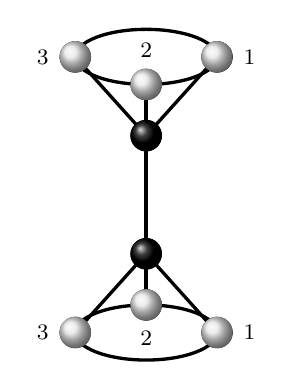
\begin{tikzpicture}[very thick, baseline=(current bounding box), font=\footnotesize]
            \draw (0, 1.5) -- (-0.9, 2.5);
            \draw (0, 1.5) -- (0.9, 2.5);
            \draw (0, 1.5) -- (0, 2.15);
            \draw (0, 2.5) circle [x radius = 0.9, y radius = 0.35];
            
            \draw (0, 0) -- (-0.9, -1);
            \draw (0, 0) -- (0.9, -1);
            \draw (0, 0) -- (0, -0.65);
            \draw (0, -1) circle [x radius = 0.9, y radius = 0.35];
            
            \draw (0, 0) -- (0, 1.5);
            
            \fill[ball color=black] (0, 0) circle [radius = 0.2];
            \fill[ball color=black] (0, 1.5) circle [radius = 0.2];
            
            \fill[ball color=black!10] (-0.9, 2.5) circle [radius = 0.2];
            \fill[ball color=black!10] (0.9, 2.5) circle [radius = 0.2];
            \fill[ball color=black!10] (0, 2.15) circle [radius = 0.2];
            
            \fill[ball color=black!10] (-0.9, -1) circle [radius = 0.2];
            \fill[ball color=black!10] (0.9, -1) circle [radius = 0.2];
            \fill[ball color=black!10] (0, -0.65) circle [radius = 0.2];
            
            \node[right] at (1.1, 2.5) {1};
            \node[above] at (0, 2.35) {2};
            \node[left] at (-1.1, 2.5) {3};
            \node[right] at (1.1, -1) {1};
            \node[below] at (0, -0.85) {2};
            \node[left] at (-1.1, -1) {3};
        \end{tikzpicture}
        \caption{Ethane molecule.}
        \label{fig:ethane molecule}
    \end{figure}
    
    \chapter{Permutation Groups}
    \section{Symmetric Group}
    \begin{dfn}{Permutation}{}
        a \defineindex{permutation}, \(\sigma\), on \(n\) objects is a bijection \(\sigma \colon X \to X\) where \(\abs{X} = n\).
    \end{dfn}
    
    Typically we identify \(X\) as \(\{1, \dotsc, n\}\).
    
    \begin{dfn}{Symmetric Permutation Group}{}
        The \defineindex{symmetric group} on \(n\) objects is the set of all permutations on \(n\) objects with function composition as a group operation.
        This group is denoted \(S_n\).
    \end{dfn}

    The order of \(S_n\) is \(n!\), since we can choose to permute the first element to any of \(n\) possible options, the second to any of \(n - 1\) options, and so on giving \(n(n - 1) \dotsm 1 = n!\) choices.
    
    \begin{lma}{}{}
        The symmetric group on \(n\) objects is a group.
        \begin{proof}
            Let \(\sigma, \rho \in S_n\).
            Then both of these are bijections on some set \(X\) with \(\abs{X} = n\).
            Their composition is defined by \((\sigma \circ \rho)(x) = \sigma(\rho(x))\) for all \(x \in X\).
            Straight away we see that this is indeed a permutation, since \(\sigma \circ \rho \colon X \to X\) and the inverse is \(\rho^{-1} \circ \sigma^{-1}\), the existence of said inverses in \(S_n\) is guaranteed as \(\sigma \in S_n\) is a bijection and so its inverse exists and is also a bijection.
            This shows that \(S_n\) is closed.
            
            The identity function, \(\mathrm{id}_X \colon X \to X\) defined by \(\mathrm{id}_X(x) = x\) for all \(x \in X\) is a permutation and \(\mathrm{id}_X \circ \sigma = \sigma\) for all \(\sigma \in S_n\).
            As previously discussed \(\sigma\) has the inverse \(\sigma^{-1}\), which is such that \(\sigma\circ \sigma^{-1} = \mathrm{id}_X\).
            Hence \(S_n\) is a group.
        \end{proof}
    \end{lma}
    
    \(S_n\) acts on the set of all tuples \((x_1, \dotsc, x_n)\) where \(x_i \in X\) are distinct in the obvious way, namely by permuting the elements:
    \begin{equation}
        \sigma \action (x_1, \dotsc, x_n) = (\sigma(x_1), \dotsc, \sigma(x_n)).
    \end{equation}
    
    \begin{dfn}{Cycle}{}
        A \(k\)-\defineindex{cycle} is a way of writing a certain permutation.
        Namely \((a_1, \dotsc, a_k)\) with \(a_i \in X\) is the permutation that sends \(a_1\) to \(a_2\), \(a_2\) to \(a_3\), and so on until \(a_{k-1}\) to \(a_k\) and \(a_k\) to \(a_1\).
        All \(x \in X\) such that \(x \ne a_i\) are left unchanged.
        
        A 2-cycle is also called a \defineindex{transposition}.
        
        The identity is usually written as \(()\) when using cycle notation, although we could also write it as a 1-cycle, \((a)\) for any \(a \in X\).
        
        Given a \(k\)-cycle \((a_1, \dotsc, a_k)\) we can start on any element of this cycle, so this is equivalent to \((a_m, \dotsc, a_k, a_1, \dotsc, a_{m-1})\).
    \end{dfn}
    
    \begin{figure}
        \tikzsetnextfilename{cycle}
        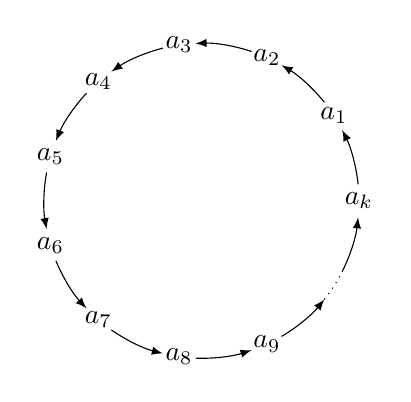
\begin{tikzpicture}
            \foreach \a in {1, ..., 9} {
                \node (a\a) at (360*\a/11:2) {\(a_{\a}\)};
                \draw[->] (360*\a/11+6:2) arc(360*\a/11+6:{360*(\a+1)/11-6}:2);
            }
            \coordinate (a10) at (3600/11:2);
            \draw[dotted] (3600/11-6:2) arc(3600/11-6:3600/11+6:2);
            \draw[->] (3600/11+6:2) arc(3600/11+6:3960/11-6:2);
            \node (al) at (3960/11:2) {\(a_k\)};
            \draw[->] (3960/11+6:2) arc(3960/11+6:4320/11-6:2);
        \end{tikzpicture}
        \caption{The \(k\)-cycle \((a_1, \dotsc, a_k)\).}
    \end{figure}
    
    \begin{exm}{}{}
        Consider \(S_4\), this contains the 3-cycles \((1, 4, 2)\) and \((1, 2, 3)\).
        We can work out their product by considering their action on some 4-tuple \((a, b, c, d)\):
        \begin{align}
            (1, 4, 2)(1, 2, 3) \action (a, b, c, d) &= (1, 4, 2) \action (c, a, b, d)\\
            &= (a, d, b, c)\\
            &= (2, 3, 4) \action (a, b, c, d),
        \end{align}
        hence, we have \((1, 4, 2) (1, 2, 3) = (2, 3, 4)\).
    \end{exm}
    
    \begin{dfn}{Disjoint Cycles}{}
        Two cycles are disjoint if no element of \(X\) appears in both cycles.
    \end{dfn}
    
    \begin{lma}{}{}
        All permutations can be written as a product of disjoint cycles.
        
        \begin{proof}
            We proceed by induction on the size of \(n = \abs{X}\).
            Clearly if \(n = 1\) then the only permutation is the identity, \(()\).
            
            Let \(\sigma \in S_n\) and suppose that all cycles in \(S_{n-1}\) can be written as disjoint cycles.
            For simplicity we will take \(X = \{1, \dotsc, n\}\).
            If \(\sigma(n) = n\) then we can consider \(\sigma\) as a permutation on \(\{1, \dotsc, n - 1\}\) leaving \(n\) fixed and we are done since this can be written as a product of disjoint cycles.
            If \(\sigma(n) = k \ne n\) then consider the permutation \(\rho = (n, k) \sigma\).
            We have that \(\rho(n) = (n, k)\sigma(n) = (n, k)k = n\).
            So we can think of \(\rho\) as being a permutation on \(\{1, \dotsc, n - 1\}\), and hence can be written as a product of disjoint cycles, \(\rho = \tau_1\dotsm \tau_r\).
            The cycles \(\tau_i\) only contain the numbers \(1, \dotsc, n -1\), and each appears in at most one of these cycles.
            
            Clearly \((n, k)(n, k) = ()\), and so it follows that
            \(\sigma = (n, k)(n, k)\sigma = (n, k)\tau_1\dotsm \tau_r\).
            If \(k\) doesn't appear in any of the cycles \(\tau_i\) then we are done as this is a product of disjoint cycles.
            Disjoint cycles commute, since by being disjoint they act on different elements of the tuple \((x_1, \dotsc, x_n)\), and so don't interact, meaning the order doesn't matter.
            Using this we are free to assume that the cycle in which \(k\) appears, if it appears, is \(\tau_1\).
            
            We are free to start on any element of the cycle so we write \(\tau_1 = (k, a_1, \dotsc, a_m)\).
            We then have
            \begin{equation}
                (n, k)\tau_1 = (n, k)(k, a_1, \dotsc, a_m) = (n, k, a_1, \dotsc, a_m).
            \end{equation}
            This follows by considering \((n, k)\tau_1(k) = (n, k)a_1 = a_1\), \((n, k)\tau_1(n) = (n, k)n = k\), \((n, k)\tau_1(a_m) = (n, k)k = n\), and \((n, k)\tau_1(a_i) = (n, k)a_{i+1} = a_{i+1}\) for \(i \ne m\).
            It follows then that we can write
            \begin{equation}
                \sigma = (n, k, a_1, \dotsc, a_m)\tau_2\dotsm \tau_r
            \end{equation}
            which is a product of disjoint cycles.
            
            Hence by induction we can write any permutation in \(S_n\) as a product of disjoint cycles for all \(n \in \naturals\).
        \end{proof}
    \end{lma}
    
    One question that we may reasonably ask is how many \(m\)-cycles are there in \(S_n\) for some fixed \(m \in \{1, \dotsc, n\}\).
    If the order of a cycle didn't matter then there would be \(\binom{n}{m}\) \(m\)-cycles in \(S_n\).
    However, the order does matter.
    Suppose we have chosen our \(m\) terms to appear in the cycle.
    We can start with any of them, reducing the number of choices that give distinct cycles by a factor of \(1/m\).
    There are then \((m - 1)!\) choices for ordering the \(m - 1\) elements remaining, giving the number of \(m\)-cycles to be
    \begin{equation}
        \binom{n}{m} \frac{1}{m} (m - 1)! = \frac{n!}{(n - m)!m!}\frac{1}{m} (m - 1)! = \frac{n!}{(n - m)!}
    \end{equation}
    where we have used \(m(m - 1)! = m!\).
    
    \begin{thm}{}{}
        The transpositions generate \(S_n\).
        That is, all permutations can be written as a product of 2-cycles.
        
        \begin{proof}
            All elements of \(S_n\) are simply \(k\)-cycles for some \(k \in \{1, \dotsc, n\}\).
            An arbitrary \(k\)-cycle can be written as
            \begin{equation}
                (a_1, a_2, \dotsc, a_k) = (a_1, a_k)(a_1, a_{k-1}) \dotsm (a_1, a_2).
            \end{equation}
            To see why this works we consider three cases.
            First, if this acts on some \(a_i\) with \(i \ne 1\), on the left hand side we clearly see that \(a_i\) maps to \(a_{i + 1}\).
            On the right hand side \(a_{i}\) commutes with cycles until a cycle with \(a_{i}\) occurs, this cycle will be \((a_1, a_i)\), and so \(a_i\) will be sent to \(a_1\).
            The next cycle is then \((a_1, a_{i + 1})\), and hence \(a_1\) maps to \(a_{i + 1}\) which then commutes with all of the remaining cycles.
            Hence \(a_i\) will map to \(a_{i+1}\).
            
            The second case is when this acts on \(a_1\), in which case the first cycle sends \(a_1\) to \(a_2\), which then commutes with all remaining cycles and so \(a_1\) maps to \(a_2\), which is what we want.
            
            The final case is trivial, its where this acts on some \(a \ne a_i\) for any \(i\), in which case on both the left and right this element is not changed and we are finished.
        \end{proof}
    \end{thm}
    
    The above theorem is fairly obvious.
    It states that we can do any permutation just by swapping two items at a time.
    This is demonstrated in \cref{fig:permutation transposition}.
    
    \begin{figure}
        \tikzsetnextfilename{permutation-by-transpositions}
        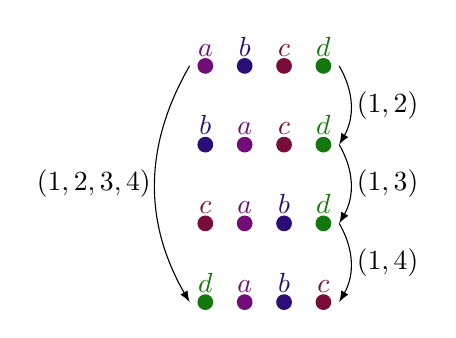
\begin{tikzpicture}
            \fill[highlight] (0, 0) circle [radius = 0.1] node[above] {\(a\)};
            \fill[my blue] (0.5, 0) circle [radius = 0.1] node[above] {\(b\)};
            \fill[my red] (1, 0) circle [radius = 0.1] node[above] {\(c\)};
            \fill[my green] (1.5, 0) circle [radius = 0.1] node[above] {\(d\)};
            
            \begin{scope}[yshift=-1cm]
                \fill[highlight] (0.5, 0) circle [radius = 0.1] node[above] {\(a\)};
                \fill[my blue] (0, 0) circle [radius = 0.1] node[above] {\(b\)};
                \fill[my red] (1, 0) circle [radius = 0.1] node[above] {\(c\)};
                \fill[my green] (1.5, 0) circle [radius = 0.1] node[above] {\(d\)};
            \end{scope}
            
            \begin{scope}[yshift=-2cm]
                \fill[highlight] (0.5, 0) circle [radius = 0.1] node[above] {\(a\)};
                \fill[my blue] (1, 0) circle [radius = 0.1] node[above] {\(b\)};
                \fill[my red] (0, 0) circle [radius = 0.1] node[above] {\(c\)};
                \fill[my green] (1.5, 0) circle [radius = 0.1] node[above] {\(d\)};
            \end{scope}
            
            \begin{scope}[yshift=-3cm]
                \fill[highlight] (0.5, 0) circle [radius = 0.1] node[above] {\(a\)};
                \fill[my blue] (1, 0) circle [radius = 0.1] node[above] {\(b\)};
                \fill[my red] (1.5, 0) circle [radius = 0.1] node[above] {\(c\)};
                \fill[my green] (0, 0) circle [radius = 0.1] node[above] {\(d\)};
            \end{scope}
            
            \draw[->] (1.7, 0) to[bend left] (1.7, -1);
            \node[right] at (1.8, -0.5) {\((1, 2)\)};
            \draw[->] (1.7, -1) to[bend left] (1.7, -2);
            \node[right] at (1.8, -1.5) {\((1, 3)\)};
            \draw[->] (1.7, -2) to[bend left] (1.7, -3);
            \node[right] at (1.8, -2.5) {\((1, 4)\)};
            
            \draw[->] (-0.2, 0) to[bend right] (-0.2, -3);
            \node[left] at (-0.57, -1.5) {\((1, 2, 3, 4)\)};
        \end{tikzpicture}
        \caption{The permutation \((1, 2, 3, 4)\) acts \((a, b, c, d)\), which can be done in steps where each step is a transposition.}
        \label{fig:permutation transposition}
    \end{figure}
    
    Notice that this theorem implies that the rank of \(S_n\) is at most \(\binom{n}{2}\), although we will see it is less than this.
    
    %   Appdendix
    \appendixpage
    \begin{appendices}
        \chapter{Mathematical Preliminaries}
\section{Basic Mathematics}
\subsection{Notation}
\begin{ntn}{Number Sets}{}
    The set of natural numbers is
    \begin{equation}
        \naturals \coloneqq \{0, 1, 2, \dotsc\}.
    \end{equation}
    Note that the inclusion of zero in \(\naturals\) is subject to debate.
    The set of integers is denoted
    \begin{equation}
        \integers \coloneqq \{\dotsc, -2, -1, 0, 1, 2, \dotsc\}.
    \end{equation}
    The set of positive integers is denoted
    \begin{equation}
        \positiveintegers \coloneqq \{1, 2, \dotsc\}.
    \end{equation}
    The set of rational numbers is denoted
    \begin{equation}
        \rationals \coloneqq \{p/q \mid p, q \in \integers \text{ and } q \ne 0\}.
    \end{equation}
    The set of real numbers is denoted \(\reals\), and the set of complex numbers \(\complex\).
    The set of \emph{all} quaternions (as opposed to the quaternion group of order 8) is denoted \(\quaternions\).
\end{ntn}

\begin{ntn}{Sphere}{}
    The unit sphere in \(n + 1\) dimensions is
    \begin{equation}
        S^n \coloneqq \{\vv{x} \in \reals^{n+1} \mid x_1^2 + \dotsb x_{n+1}^2 = 1\}.
    \end{equation}
    Note that \(S^n\) is an \(n\)-dimensional manifold, which we view as embedded in \((n + 1)\)-dimensional Euclidean space, \(\reals^{n+1}\).
    
    What we normally call the circle is \(S^1\) and what we normally call the sphere is \(S^2\).
\end{ntn}

\begin{ntn}{Sets of Matrices}{}
    We denote the set of \(m \times n\) matrices with entries in \(\field\) (which is usually a field and usually \(\reals\) or \(\complex\)) by \(\matrices[m]{n}{\field}\).
    
    We denote the set of square \(n \times n\) matrices with entries in \(\field\) by \(\matrices{n}{\field}\).
    
    We denote the set of invertible \(n\times n\) square matrices over \(\field\), called the general linear group, by
    \begin{equation}
        \generalLinear(n, \field) = \{A \in \matrices{n}{\field} \mid \det A \ne 0\}.
    \end{equation}
    If \(\field\) is evident from context we may simply write \(\generalLinear(n)\).
    If \(V\) is an \(n\)-dimensional vector space over \(\field\) then we may also write this set as \(\generalLinear(V)\).
\end{ntn}

\begin{ntn}{Einstein Summation Convention}{}
    When two identical indices appear in the same term then they are summed over, for example,
    \begin{equation}
        x_iy_i = \sum_{i} x_iy_i.
    \end{equation} 
\end{ntn}

\subsection{Definitions}
\begin{dfn}{Function Types}{}
    Let \(\varphi \colon A \to B\).
    Then \(\varphi\) is 
    \begin{itemize}
        \item \defineindex{injective} if for all \(a, a' \in A\) \(\varphi(a) = \varphi(a')\) implies \(a = a'\),
        \item \defineindex{surjective} if for all \(b \in B\) there exists \(a \in A\) such that \(\varphi(a) = b\), and
        \item \defineindex{bijective} if \(\varphi\) is both injective and surjective.
    \end{itemize}
    A function is invertible if and only if it is bijective.
\end{dfn}

\begin{figure}
    \begin{subfigure}[t]{0.45\textwidth}
        \centering
        \tikzsetnextfilename{injective-function}
        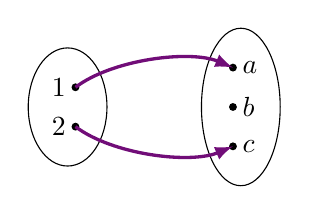
\begin{tikzpicture}
            \foreach \y in {-0.5, 0, 0.5} {
                \fill (2, \y) circle [radius = 0.05cm];
            }
            \foreach \y in {-0.25, 0.25} {
                \fill (0, \y) circle [radius = 0.05cm];
            }
            \node [right] at (2, -0.5) {\(c\)};
            \node [right] at (2, 0) {\(b\)};
            \node [right] at (2, 0.5) {\(a\)};
            \node [left] at (0, -0.25) {\(2\)};
            \node [left] at (0, 0.25) {\(1\)};
            \draw (-0.1, 0) circle [x radius = 0.5, y radius = 0.75];
            \draw (2.1, 0) circle [x radius = 0.5, y radius = 1];
            
            \draw [very thick, highlight, ->] (0, 0.25) to[bend left, looseness=0.75] (2, 0.5);
            \draw [very thick, highlight, ->] (0, -0.25) to[bend right, looseness=0.75] (2, -0.5);
        \end{tikzpicture}
        \caption{An injective function, \(f \colon \{1, 2\} \to \{a, b, c\}\). Note that \(f(x) \ne b\) for any \(x \in \{1, 2\}\) and so the function fails to be surjective.}
    \end{subfigure}
    \hspace{0.05\textwidth}
    \begin{subfigure}[t]{0.45\textwidth}
        \centering
        \tikzsetnextfilename{surjective-function}
        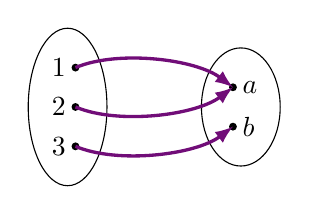
\begin{tikzpicture}
            \foreach \y in {-0.5, 0, 0.5} {
                \fill (0, \y) circle [radius = 0.05cm];
            }
            \foreach \y in {-0.25, 0.25} {
                \fill (2, \y) circle [radius = 0.05cm];
            }
            \node [left] at (0, -0.5) {\(3\)};
            \node [left] at (0, 0) {\(2\)};
            \node [left] at (0, 0.5) {\(1\)};
            \node [right] at (2, -0.25) {\(b\)};
            \node [right] at (2, 0.25) {\(a\)};
            \draw (-0.1, 0) circle [x radius = 0.5, y radius = 1];
            \draw (2.1, 0) circle [x radius = 0.5, y radius = 0.75];
            
            \draw [very thick, highlight, ->] (0, 0.5) to[bend left, looseness=0.75] (2, 0.25);
            \draw [very thick, highlight, ->] (0, 0) to[bend right, looseness=0.75] (2, 0.25);
            \draw [very thick, highlight, ->] (0, -0.5) to[bend right, looseness=0.75] (2, -0.25);
        \end{tikzpicture}
        \caption{A surjective function, \(g \colon \{1, 2, 3\} \to \{a, b\}\). Note that \(g(1) = g(2)\) but \(1 \ne 2\) and so the function fails to be injective.}
    \end{subfigure}
    \begin{subfigure}[t]{0.5\textwidth}
        \centering
        \tikzsetnextfilename{bijective-function}
        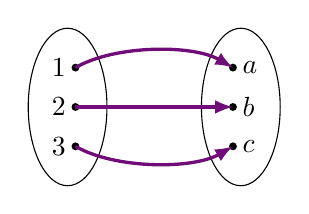
\begin{tikzpicture}
            \foreach \y in {-0.5, 0, 0.5} {
                \fill (0, \y) circle [radius = 0.05cm];
            }
            \foreach \y in {-0.5, 0, 0.5} {
                \fill (2, \y) circle [radius = 0.05cm];
            }
            \node [left] at (0, -0.5) {\(3\)};
            \node [left] at (0, 0) {\(2\)};
            \node [left] at (0, 0.5) {\(1\)};
            \node [right] at (2, 0.5) {\(a\)};
            \node [right] at (2, 0) {\(b\)};
            \node [right] at (2, -0.5) {\(c\)};
            \draw (-0.1, 0) circle [x radius = 0.5, y radius = 1];
            \draw (2.1, 0) circle [x radius = 0.5, y radius = 1];
            
            \draw [very thick, highlight, ->] (0, 0.5) to[bend left, looseness=0.75] (2, 0.5);
            \draw [very thick, highlight, ->] (0, 0) -- (2, 0);
            \draw [very thick, highlight, ->] (0, -0.5) to[bend right, looseness=0.75] (2, -0.5);
        \end{tikzpicture}
        \caption{A bijective function, \(h \colon \{1, 2, 3\} \to \{a, b, c\}\).}
    \end{subfigure}
    \caption{Injective, surjective, and bijective functions.}
\end{figure}

\begin{dfn}{Kernel}{}
    Given a map \(\varphi \colon A \to B\) the \defineindex{kernel} is defined as the set of elements of \(A\) which map to the trivial element of \(B\), which is the zero vector, \(\vv{0}\), if \(B\) is a vector space, or the identity if \(B\) is a group:
    \begin{equation}
        \ker\varphi \coloneqq \{a \in A \mid \varphi(a) \text{ is the trivial element of \(B\)}\} \subseteq A.
    \end{equation}
\end{dfn}

\begin{dfn}{Image}{}
    Given a map \(\varphi \colon A \to B\) the \defineindex{image} is set of \(b \in B\) for which there exists some \(a \in A\) such that \(\varphi(a) = b\):
    \begin{equation}
        \image\varphi = \varphi(A) \coloneqq \{b \in B \mid \exists \, a \in A \text{ such that } \varphi(a) = b\} \subseteq B.
    \end{equation}
\end{dfn}

\begin{dfn}{Empty Set}{}
    The \defineindex{empty set}, \(\emptyset\), is the set containing no elements.
\end{dfn}

\begin{dfn}{Kronecker Delta}{}
    The \defineindex{Kronecker delta}, \(\delta_{ij}\), is defined as
    \begin{equation}
        \delta_{ij} \coloneqq
        \begin{cases}
            1, & \text{if } i = j,\\
            0, & \text{if } i \ne j.
        \end{cases}
    \end{equation}
    Note that \(\delta_{ij}\) are the elements of the identity matrix.
\end{dfn}

\begin{dfn}{Levi-Civita Symbol}{}
    The \defineindex{Levi-Civita Symbol} in \(n\)-indices is the completely asymmetric (pseudo)tensor which is defined so that \(\varepsilon_{123\dotso n} \coloneqq 1\).
    Antisymmetry then means that \(\varepsilon_{1\dotsm i\dotsm j \dotsm n} = -\varepsilon_{1\dotsm j\dotsm i\dotsm n}\), for example \(\varepsilon_{213\dotsm n} = -1\).
    Antisymmetry also means that Levi--Civita symbol vanishes if it has repeated indices.
    
    Most commonly \(n = 3\) and
    \begin{equation}
        \varepsilon_{ijk} \coloneqq 
        \begin{cases}
            1, & \text{if } (i, j, k) = (1, 2, 3), (2, 3, 1), (3, 1, 2),\\
            -1, & \text{if } (i, j, k) = (1, 3, 2), (2, 1, 3), (3, 2, 1),\\
            0, & \text{if any index is repeated}.
        \end{cases}
    \end{equation}
\end{dfn}

\begin{dfn}{Equivalence Relations}{}
    Given two sets, \(A\) and \(B\), a \defineindex{relation}, \(R\), is a subset of \(A \times B \coloneqq \{(a, b) \mid a \in A \text{ and } b \in B\} \supseteq R\).
    We say that \(a \in A\) is related to \(b \in B\), which we denote with infix notation, \(a\mathbin{R}b\), if \((a, b) \in R\).
    
    If \(A = B\) in the above definition then we call \(R\) a \defineindex{binary!relation} on \(A\).
    
    A relation, \(\sim\), on a set \(A\) is a binary relation on \(A\) such that the following axioms hold for all \(a, b, c \in A\)
    \begin{itemize}
        \item \(\sim\) is \defineindex{reflexive}, so \(a \sim a\).
        \item \(\sim\) is \define{symmetric}\index{symmetric!relation}, so if \(a \sim b\) then \(b \sim a\).
        \item \(\sim\) is \defineindex{transitive}, so if \(a \sim b\) and \(b \sim c\) then \(a \sim c\).
    \end{itemize}
    
    An \defineindex{equivalence class} of an element \(a \in A\) under some equivalence relation, \(\sim\), is the set
    \begin{equation}
        [a] \coloneqq \{x \mid a \sim x\}.
    \end{equation}
    We call elements of \([a]\) representatives of the equivalence class.
    We denote the set of all equivalence classes by \(A/\sim\).
\end{dfn}

\begin{exm}{Equivalence Relations}{}
    \(=\) is the prototypical equivalence relation.
    
    Congruence modulo \(m \in \positiveintegers\) is an equivalence relation on \(\reals\).
    
    \(\sim\) defined by \(z\sim w\) if \(\abs{z} = \abs{w}\) is an equivalence relation on \(\complex\).
    
    \(\sim\) defined by \(\vv{v} \sim \vv{u}\) if \(\vv{u}\) and \(\vv{v}\) are parallel is an equivalence relation on \(\reals^n\).
\end{exm}

\begin{exm}{Isomorphism}{exm:isomorphism is equivalence relation}
    Isomorphisms, as defined in the text, are equivalence relations:
    \begin{itemize}
        \item Let \(A\) be a group, then the identity function, \(\mathrm{id}_A\colon A \to A\) defined by \(\mathrm{id}_A(a) = a\) for all \(a \in A\) is an isomorphism since \(\mathrm{id}_A(aa') = aa' = \mathrm{id}_A(a)\mathrm{id}_A(a')\) and clearly \(\mathrm{id}_A\) is invertible, and is its own inverse.
        \item Let \(A\) and \(B\) be isomorphic groups.
        Then there exists some bijection \(\varphi \colon A \to B\) such that \(\varphi(aa') = \varphi(a)\varphi(a')\).
        Since \(\varphi\) is a bijection \(\varphi^{-1}\colon B \to A\) exists and is also a bijection.
        Applying the inverse to both sides of the defining relation we have \(\varphi^{-1}(\varphi(aa')) = \varphi^{-1}(\varphi(a)\varphi(a'))\).
        Since \(\varphi\) is surjective any element of \(B\) can be written in the form \(b = \varphi(a)\) for some \(a \in A\) and so it follows that \(\varphi^{-1}(\varphi(aa')) = \varphi^{-1}(b)\varphi(b')\) where \(b, b' \in B\) are arbitrary, and we choose \(a, a' \in A\) to be such that \(b = \varphi(a)\) and \(b' = \varphi(a')\).
        From the defining relation for \(\varphi\) we know that \(\varphi(aa') = \varphi(a)\varphi(a') = bb'\).
        It follows that \(\varphi^{-1}(\varphi(aa')) = \varphi^{-1}(bb') = \varphi^{-1}(b)\varphi^{-1}(b')\), which means that \(B \isomorphic A\).
        \item Let \(A\), \(B\), and \(C\) be groups such that \(A \isomorphic B\) and \(B \isomorphic C\).
        Then there exists isomorphisms \(\varphi \colon A \to B\) and \(\psi\colon B \to C\).
        We claim that \(\psi\circ \varphi \colon A \to C\) is an isomorphism.
        Clearly \(\psi\circ \varphi\) is bijective, since \(\varphi^{-1}\circ \psi^{-1}\) is its inverse, as can be seen by considering \((\varphi^{-1}\circ \psi^{-1})((\psi\circ \varphi)(a)) = \varphi^{-1}(\psi^{-1}(\psi(\varphi(a)))) = \varphi^{-1}(\varphi(a)) = a\) for all \(a \in A\).
        
        It remains to show that \(\psi \circ \varphi\) is a homomorphism.
        To do so consider \((\psi \circ \varphi)(aa') = \psi(\varphi(aa')) = \psi(\varphi(a)\varphi(a'))\), which follows since \(\varphi\) is an isomorphism.
        Now write \(\varphi(a) = b\) and \(\varphi(a') = b'\), where \(b, b' \in B\).
        We then have \((\psi \circ \varphi)(aa') = \psi(bb') = \psi(b)\psi(b')\), which follows since \(\psi\) is an isomorphism.
        We then have \((\psi \circ \varphi)(aa') = \psi(b)\psi(b') = \psi(\varphi(b))\psi\varphi(b') = (\psi \circ \varphi)(b)(\psi \circ \varphi)(b')\), and so \(\psi\circ\varphi\) is a bijective homomorphism and hence an isomorphism, meaning \(A \isomorphic C\).
    \end{itemize}
\end{exm}

\section{Linear Algebra}
\subsection{Vectors}
\begin{dfn}{Vector Space}{}
    A vector space, \(V\), over a field, \(\field\), is a set of vectors, \(V\), with two operations, \(\cdot\colon \field \times V \to V\), known as scalar multiplication, and \(+\colon V\times V \to V\), known as vector addition, which are defined such that the following hold for all \(\vv{u}, \vv{v}, \vv{w} \in V\) and \(k, k' \in \field\):
    \begin{enumerate}
        \item \define{Associativity}\index{accociative}: \(\vv{u} + (\vv{v} + \vv{w}) = (\vv{u} + \vv{v}) + \vv{w}\),
        \item There exists a \define{zero vector}, \(\vv{0} \in V\), such that \(\vv{u} + \vv{0} = \vv{u}\).
        \item There exists \(-\vv{u} \in V\) such that \(\vv{u} + (-\vv{u}) = \vv{0}\).
        We write this as \(\vv{u} - \vv{u}\) for short.
        \item \define{Commutativity}\index{commutative}: \(\vv{u} + \vv{v} = \vv{v} + \vv{u}\).
        \item Distributivity of scalar multiplication over vector addition \(k(\vv{u} + \vv{v}) = k\vv{u} + k\vv{v}\).
        \item Distributivity of scalar multiplication over field addition \((k + k')\vv{u} = k\vv{u} + k'\vv{u}\).
        \item Compatibility of field and scalar multiplication \((kk')\vv{u} = k(k'\vv{u})\).
        \item \(1\vv{u} = \vv{u}\) where \(1\) is the multiplicative identity of \(\field\).
    \end{enumerate}
    Note that the first three axioms make \((V, +)\) a group and the fourth makes it Abelian.
\end{dfn}

\begin{dfn}{Hilbert Space}{}
    A \defineindex{Hilbert space}, \(\hilbert\), is a vector space over either \(\reals\) or \(\complex\), equipped with an inner product that induces a complete metric.
    We shall assume a complex Hilbert space, for a real Hilbert space simply ignore any complex conjugates and replace \(\complex\) with \(\reals\).
    
    An \defineindex{inner product}\index{\(\innerprod{-}{-}\), inner product} is a function \(\innerprod{-}{-} \colon \hilbert \times \hilbert \to \complex\) such that for all \(\vv{u}, \vv{v}, \vv{w} \in \hilbert\) and \(k, k' \in \complex\)
    \begin{enumerate}
        \item \(\innerprod{-}{-}\) is linear in its second argument, that is
        \begin{equation}
            \innerprod{\vv{u}}{k\vv{v} + k'\vv{w}} = k\innerprod{\vv{u}}{\vv{v}} + k'\innerprod{\vv{u}}{\vv{w}}.
        \end{equation}
        \item \(\innerprod{-}{-}\) is conjugate symmetric:
        \begin{equation}
            \innerprod{\vv{u}}{\vv{v}} = \innerprod{\vv{v}}{\vv{u}}^*.
        \end{equation}
        \item \(\innerprod{-}{-}\) is positive definite, that is \(\innerprod{\vv{u}}{\vv{u}} \ge 0\) with equality only if \(\vv{u} = \vv{0}\).
    \end{enumerate}
    \begin{wrn}
        Mathematicians often define an inner product to be linear in its first argument, so
        \begin{equation}
            \innerprod{k\vv{u} + k'\vv{v}}{\vv{w}} = k\innerprod{\vv{u}}{\vv{w}} + k'\innerprod{\vv{v}}{\vv{w}}.
        \end{equation}
    \end{wrn}
    The first two axioms are sometimes combined to give an extra axiom that \(\innerprod{-}{-}\) is conjugate linear in its first argument (or second if we follow the other convention).
    That is
    \begin{equation}
        \innerprod{k\vv{u} + k'\vv{v}}{\vv{w}} = k^*\innerprod{\vv{u}}{\vv{w}} + k'^*\innerprod{\vv{v}}{\vv{w}}.
    \end{equation}
    We can then define a \defineindex{norm}\index{\(\norm{-}\), norm} on \(\hilbert\) by \(\norm{\vv{u}} \coloneqq \sqrt{\innerprod{\vv{u}}{\vv{u}}}\).
    
    The final condition for \(\hilbert\) to be a Hilbert space is completeness.
    Namely, that if the series \(\sum_{n=0}^{\infty} \vv{u_n}\) converges absolutely, so that \(\sum_{n=0}^{\infty} \norm{\vv{u_n}}\) converges to a finite value then the original series, \(\sum_{n=0}^{\infty} \vv{u_n}\), converges to some vector in \(\hilbert\).
\end{dfn}

\begin{exm}{}{}
    The set of \(n\)-tuples of complex numbers, \(\complex^n\), is a Hilbert space over \(\complex\) with the inner product
    \begin{equation}
        \innerprod{\vv{u}}{\vv{v}} = \innerprod{(u_1, \dotsc, u_n)}{(v_1, \dotsc, v_n)} \coloneqq \sum_{i=1}^n u_i^*v_i = u_i^*v_i
    \end{equation}
    where in the last term we use the Einstein summation convention.
\end{exm}

\begin{exm}{Functions}{}
    The space of square integrable functions on \(X \subseteq \reals^n\) forms a Hilbert space, denoted \(L^2(X)\).
    A function, \(f\colon X \to \complex\), is square integrable if\footnote{For this space to be complete (a requirement for Hilbert spaces) this must be a Lebesgue integral but in physics functions are usually nice enough that we can use the standard Riemann integral, which agrees with the Lebesgue integral when both exists.}
    \begin{equation}
        \int_{X} \abs{f(x)}^2 \dd{x}
    \end{equation}
    exists and is finite.
    For example, the function defined by \(f(x) = e^{-x^2}\) is an element of \(L^2(\reals)\).
    
    Given \(f, g \in L^2(X)\) we define the inner product in this space to be
    \begin{equation}
        \innerprod{f}{g} \coloneqq \int_{X} f^*(x)g(x) \dd{x}.
    \end{equation}
    \begin{rmk}
        Another subtly that arises here is that we actually need to consider elements of \(L^2(X)\) to be equivalence classes of functions which are equal almost everywhere (meaning that the measure of the set of points where they are not equal is zero).
        Otherwise, we may have some functions such that \(\innerprod{f}{g} = 0\) but \(f \ne g\) since \(f\) and \(g\) disagree on some set of points with a vanishing measure.
        We say that we are considering the functions mod the equivalence relation of being equal almost everywhere.
    \end{rmk}
    
    This is an important example since we can often identify \enquote{square integrable functions} with \enquote{possible wave functions}, since square-integrability is a requirement for us to be able to normalise a wave function, which we do so by the procedure
    \begin{equation}
        \psi \to \frac{\psi}{\norm{\psi}} = \frac{\psi}{\sqrt{\innerprod{\psi}{\psi}}} = \left( \int \abs{\psi(x)}^2 \dd{x} \right)^{-1/2} \psi.
    \end{equation}
    This only makes sense if \(\int \abs{\psi(x)}^2 \dd{x}\) is finite (and nonzero).
\end{exm}

\begin{ntn}{Bra-Ket Notation}{}
    In physics, particularly in quantum mechanics, we often use \defineindex{bra-ket notation}, developed by Dirac.
    We identify vectors, \(\vv{u}\), with \define{kets}\index{ket}\index{\(\ket{-}\), ket}, \(\ket{u}\), and dual vectors, \(\vv{v}\), with \define{bras}\index{bra}\index{\(\bra{-}\), bra}, \(\bra{v}\).
    The inner product \(\innerprod{\vv{u}}{\vv{v}}\) is then written \(\braket{v}{u}\)\index{\(\braket{-}{-}\), inner product}.
    This is the notation we will use for most of this course.
\end{ntn}

\begin{dfn}{Linear Operator}{}
    Given two vector spaces, \(V\) and \(W\), over some field, \(\field\), a function, \(f \colon V \to W\), is said to be a linear operator if for \(\vv{u}, \vv{v} \in V\) and \(k \in \field\) we have
    \begin{equation}
        f(\vv{u} + \vv{v}) = f(\vv{u}) + f(\vv{v}), \qqand f(k\vv{u}) = kf(\vv{u}).
    \end{equation}
    
    Instead of the function notation \(f(\vv{u})\) we typically use a multiplicative notation, \(A\vv{u}\), which is due to the fact that if \(V\) is finite dimensional then we can choose a basis and represent a linear map by a matrix.
    Using bra-ket notation also we have
    \begin{equation}
        A(\ket{u} + \ket{v}) = A\ket{u} + A\ket{v}, \qqand A(k\ket{u}) = kA\ket{u}.
    \end{equation}
    
    An operator is \defineindex{antilinear} if
    \begin{equation}
        A(\ket{u} + \ket{v}) = A\ket{u} + A\ket{v}, \qqand A(k\ket{u}) = k^*A\ket{u}.
    \end{equation}
    An example of such an operator is the time reversal operator, \(T\), which takes \(t \to -t\).
\end{dfn}

For simplicity from now on we will consider the complex vector space \(V = \complex^N\).
This is \(N\)-dimensional (\(\dim V = N\)), which we take to be finite, although many of these ideas work, possibly with slight modification, for infinite dimensional vector spaces.
Most of the time we will also consider linear operators from \(V\) to \(V\), since this is far more common in practice that linear operators from \(V\) to some different vector space, \(W\).

\begin{dfn}{Basis}{}
    Given a vector space, \(V\), we say that \(\{\ket{e_i}\}\) is a \defineindex{linearly independent} set if the only solution to
    \begin{equation}
        \lambda_i\ket{e_i} = \ket{0},
    \end{equation}
    where \(\ket{0}\) is the zero vector, is \(\lambda_i = 0\) for all \(i\).
    
    We say that \(\{\ket{e_i}\}\) is a \defineindex{basis} for \(V\) if \(\{\ket{e_i}\}\) is a linearly independent set and spans \(V\).
    That is given some \(\ket{u} \in V\) we can write
    \begin{equation}
        \ket{u} = u_i\ket{e_i}
    \end{equation}
    for some \(u_i \in \complex\).
    
    The number of vectors in a basis is the \defineindex{dimension} of the vector space, denoted \(\dim V\)\index{dim@\(\dim\), dimension}.
    
    We say that two vectors, \(\ket{u}, \ket{v} \in V\), are \define{orthogonal}\index{orthogonal!vectors} (with respect to some inner product) if \(\braket{u}{v} = 0\).
    
    We say that a vector, \(\ket{u} \in V\), is normalised if \(\norm{u} = \sqrt{\braket{u}{u}} = 1\).
    
    We say that \(\{\ket{e_i}\}\) is an orthonormal basis for \(V\) if it is a basis for \(V\), \(\ket{e_i}\) is normalised for all \(i\) and all of the basis vectors are mutually orthogonal.
    These last two conditions are summarised by requiring that
    \begin{equation}
        \braket{e_i}{e_j} = \delta_{ij}.
    \end{equation}
\end{dfn}

\begin{dfn}{Completeness Relation}{}
    Given a vector space, \(V\), and an orthonormal basis, \(\{\ket{e_i}\}\), we can write the identity operator, \(\ident\), as
    \begin{equation}
        \ident = \sum_{i=1}^{N} \ket{e_i}\bra{e_i}.
    \end{equation}
    Recall that the identity operator is defined such that\index{\(\ident\), identity matrix}
    \begin{equation}
        \ident\ket{u} = \ket{u}
    \end{equation}
    for all \(\ket{u} \in V\).
\end{dfn}

\begin{dfn}{Partition of the Identity}{}
    A \defineindex{projection operator}, \(P_i\), is an operator satisfying
    \begin{equation}
        P_iP_j = \delta_{ij}P_i, \qqand P_i^\hermit = P_i.
    \end{equation}
    A \defineindex{partition of the identity} is a collection of projection operators, \(\{P_j\}\), such that
    \begin{equation}
        \ident = \sum_{j=1}^{N_P} P_j
    \end{equation}
    where \(N_P = \abs{\{P_j\}}\) is the number of projection operators in the partition.
    We can write each partition operator as
    \begin{equation}
        P_j = \sum_{i=1}^{N_j} \ket{e_i}\bra{e_i}
    \end{equation}
    where \(N_j\) are such that
    \begin{equation}
        \dim V = N = \sum_{j=1}^{N_P}N_j.
    \end{equation}
\end{dfn}

\begin{dfn}{Matrix Element}{}
    Given a linear operator, \(A \colon V \to V\), and an orthonormal basis, \(\{\ket{e_i}\}\), we define the \define{matrix elements}\index{matrix element} to be
    \begin{equation}
        A_{ij} \coloneqq \braket{e_i}{Ae_j} = \bra{e_i}A\ket{e_j}
    \end{equation}
    where \(A\) is understood to act on the right and \(\ket{Ae_j} \coloneqq A\ket{e_j}\).
    
    If we know the matrix elements of \(A\) we can reconstruct \(A\) using
    \begin{equation}
        A = \sum_{i=1}^{N}\sum_{j=1}^{N} A_{ij}\ket{e_i}\bra{e_j}.
    \end{equation}
\end{dfn}

\begin{dfn}{Eigenvalues and Eigenvectors}{}
    Given a linear operator \(A\), we call \(\ket{v_i}\) an \defineindex{eigenvector} and \(\lambda_i\in\complex\) an \defineindex{eigenvalue} if
    \begin{equation}
        A\ket{v_i} = \lambda_i\ket{v_i}.
    \end{equation}
    There are \(N\) solutions to this, which follows from the \define{characteristic polynomial}\index{characteristic!polynomial}, \(\det(A - \lambda\ident) = 0\), having \(N\) solutions, which in turn follows from the fundamental theorem of algebra.
\end{dfn}

\subsection{Matrices}
\begin{dfn}{Transpose and Hermitian Conjugate}{}
    Given a matrix, \(A\), with matrix elements \(A_{ij}\), the \defineindex{transpose}\index{\(-^\trans\), transpose} matrix, \(A^\trans\), has matrix elements \(A^\trans_{ij} = A_{ji}\).
    
    A matrix is \defineindex{symmetric} if \(A^\trans = A\), or \defineindex{antisymmetric} if \(A^\trans = -A\).
    
    Given a matrix, \(A\), with matrix elements \(A_{ij}\), the \defineindex{Hermitian conjugate}\index{\(-^\hermit\), Hermitian conjugate}, \(A^\hermit\), has matrix elements \(A^\hermit_{ij} = A_{ji}^*\).
    Here \(^*\) denotes the \defineindex{complex conjugate}\index{\(-^*\), complex conjugate}, so \((x + iy)^* = x - iy\) and \((r\e^{i\vartheta})^* = r\e^{-\vartheta}\) for \(x, y, r, \vartheta \in \reals\).
    That is the Hermitian conjugate is the complex conjugate of the transpose.
    
    A matrix is \defineindex{Hermitian} if \(A^\hermit = A\), or \defineindex{anti-Hermitian} if \(A^\hermit = -A\).
\end{dfn}

\begin{lma}{}{}
    The eigenvalues of a Hermitian matrix are real.
    \begin{proof}
        Let \(A\) be a Hermitian matrix and \(\vv{v}\) an eigenvector with nonzero eigenvalue \(\lambda\).
        Note that this means \(\vv{v}\) is nonzero.
        If \(0\) is an eigenvalue of \(A\) then this is real, so we need not consider this case further.
        By definition \(A\vv{v} = \lambda\vv{v}\).
        Taking the Hermitian conjugate of both sides we get \(\vv{v}^\hermit A^\hermit = \lambda^*\vv{v}^\hermit\), where we have used \((XY)^\hermit = Y^\hermit X^\hermit\).
        Multiplying both sides on the right by \(\vv{v}\) we get \(\vv{v}^\hermit A \vv{v} = \lambda^*\vv{v}^\hermit \vv{v}\).
        Identifying \(A\vv{v} = \lambda\vv{v}\) on the left-hand side this becomes \(\vv{v}^\hermit \lambda \vv{v} = \lambda\vv{v}^\hermit \vv{v} = \lambda^*\vv{v}^\hermit \vv{v}\).
        It follows that we must have \(\lambda = \lambda^*\), which means we must have \(\lambda \in \reals\).
    \end{proof}
\end{lma}

We can choose the eigenvalues of a Hermitian matrix to be orthonormal, and hence they form a basis for the vector space.
In this basis the matrix will be diagonal and the values on the diagonal are simply the eigenvalues.

Given a Hermitian matrix, \(A\), with eigenvalues \(\lambda_i\) and corresponding eigenvectors \(\ket{v_i}\) we can write this matrix as
\begin{equation}
    A = \sum_{i=1}^{N} \lambda_i\ket{v_i}\bra{v_i}.
\end{equation}
This is diagonalised by the transformation \(V^\hermit A V\) where
\begin{equation}
    V = \sum_{i=1}^{N} \ket{v_i}\bra{e_i}
\end{equation}
where \(\ket{e_i}\) are the basis vectors in the original basis.
It is easy to see that this transform gives the desired result:
\begin{align}
    V^\hermit AV &= \underbrace{\ket{e_i}\bra{v_i}}_{=V^\hermit}  \underbrace{(\lambda_j \ket{v_j}\bra{v_j})}_{=A}\underbrace{\ket{v_k}\bra{e_k}}_{=V}\\
    &= \lambda_j \ket{e_i}\braket{v_i}{v_j}\braket{v_j}{v_k}\bra{e_k}\\
    &= \lambda_j \delta_{ij}\delta_{jk} \ket{e_i}\bra{e_k}\\
    &= \lambda_i \ket{e_i}\bra{e_i}
\end{align}
This last term is just a diagonal matrix with the eigenvalues, \(\lambda_i\), as the diagonal elements, which is exactly what we wanted.

For non-Hermitian matrices it is possible that the eigenvalues aren't linearly independent.
In this case the best we can do is Jordan normal form where the eigenvalues are on the diagonal and all other entries are either zero or one for elements in the subspace of degenerate eigenvalues.

\begin{dfn}{Inverse}{}
    The \defineindex{inverse}\index{\(-^{-1}\), inverse} of a matrix, \(A\), is the matrix \(A^{-1}\) such that \(A^{-1}A = AA^{-1} = \ident\).
    Such a matrix exists only if the determinant is non-zero.
\end{dfn}

An equivalent requirement for \(A^{-1}\) to exist is for \(A\) to have no zero eigenvalues.
For a Hermitian matrix the inverse in the eigenbasis is simply \(A^{-1} = \diag(1/\lambda_1, \dotsc, 1/\lambda_N)\).

\begin{dfn}{Orthogonal and Unitary}{}
    A matrix, \(O\), is \define{orthogonal}\index{orthogonal!matrix} if \(O^\trans O = \ident\), that is \(O^\trans = O^{-1}\).
    
    A matrix, \(U\), is \defineindex{unitary} if \(U^\hermit U = \ident\), that is \(U^\hermit = U^{-1}\).
\end{dfn}

The following holds:
\begin{equation}
    \braket{u}{Av} = \bra{u}A\ket{v} = \braket{A^\hermit u}{v}.
\end{equation}
For a unitary matrix, \(U\), this implies
\begin{equation}
    \braket{Uu}{Uv} = \bra{u}U^\hermit U\ket{v} = \bra{u}\ident \ket{v} = \braket{u}{v}.
\end{equation}
We say that unitary transforms preserve the inner product, or that the inner product is invariant under unitary transforms.

\begin{dfn}{Trace}{}
    The \defineindex{trace}\index{tr@\(\tr\), trace} of a matrix, \(A\) is
    \begin{equation}
        \tr A \coloneqq \sum_{i} \bra{e_i} A_i \ket{i} = A_{ii}
    \end{equation}
    where in the last term we are using the Einstein summation convention to sum over \(i\).
\end{dfn}

The trace of a matrix is simply the sum of its eigenvalues, this doesn't just hold for Hermitian matrices.

The trace is cyclic, meaning \(\tr(AB) = \tr(BA)\), \(\tr(ABC) = \tr(BCA) = \tr(CAB)\), etc.

The trace is linear, meaning \(\tr(k A) = k\tr(A)\) for scalar \(k\).

\(\innerprod{A}{B} \coloneqq \tr(A^\hermit B)\) is an inner product on the vector space of matrices.
This is called the \defineindex{Gram--Schmidt inner product}.

\begin{dfn}{Determinant}{}
    The \defineindex{determinant}\index{det@\(\det\), determinant}\index{\(\abs{-}\), determinant} of a matrix, \(A\), is 
    \begin{equation}
        \det A = \abs{A} = \coloneqq \varepsilon_{i_1\dotso i_N} A_{1i_1}\dotsm A_{Ni_N}
    \end{equation}
    with summation over indices implied.
\end{dfn}

The determinant of a matrix is the product of its eigenvalues.

The determinant of a product is the product of the determinants:
\begin{equation}
    \det(AB) = \det(A)\det(B) = \det(B)\det(A) = \det(BA).
\end{equation}

\begin{dfn}{Diagonal}{}
    A matrix, \(A\), is \defineindex{diagonal} if \(A_{ij} = 0\) for \(i \ne j\).
    
    A matrix, \(A\), is \defineindex{block diagonal} if it can be written in the form
    \begin{equation}
        A = 
        \begin{pmatrix}
            A_1 & 0 & 0 & \dots & 0\\
            0 & A_2 & 0 & \dots & 0\\
            \vdots & \vdots & \vdots & \ddots & \vdots\\
            0 & 0 & 0 & 0 & A_n
        \end{pmatrix}
    \end{equation}
    where \(A_i\) are square matrices and the \(0\)s represent matrices where all elements are zero.
\end{dfn}    

\subsection{Combining Vector Spaces}
\begin{dfn}{Direct Sum}{dfn:direct sum}
    Given vector spaces \(V\) and \(W\) we call \(V\directsum W\)\index{\(\directsum\), direct sum} the \defineindex{direct sum}.
    It is defined by associating with each pair of vectors, \(\ket{v_i} \in V\) and \(\ket{w_a} \in W\), a vector \(\ket{v_i} \directsum \ket{w_i} = \ket{v_i \directsum w_a} \in V \directsum W\) and extending the inner product to
    \begin{equation}
        \braket{v_i \directsum w_a}{v_j \directsum w_b}_{V\directsum W} \coloneqq \braket{v_i}{v_j}_{V} + \braket{w_a}{w_b}_{W}
    \end{equation}
    where the subscripts denote which vector space the inner product is in.
    Note that the notation \(\ket{v \directsum w}\) is non-standard.
    
    The dimension of \(V \directsum W\) is
    \begin{equation}
        \dim(V \directsum W) = \dim V + \dim W.
    \end{equation}
    
    Given \(A \in \generalLinear(V)\) and \(B \in \generalLinear(W)\) the direct sum, \(A \directsum B\), acts on \(\ket{v} \directsum \ket{w} \in V \directsum W\) as
    \begin{equation}
        (A \directsum B)(\ket{v} \directsum \ket{w}) \coloneqq (A\ket{v}) \directsum (B\ket{w}).
    \end{equation}
    This shows we can think of \(V \directsum W\) as a \((\dim V + \dim W)\)-dimensional vector space with operators represented by \((v + w) \times (v + w)\) block diagonal matrices:
    \begin{equation}
        A \directsum B = 
        \begin{pmatrix}
            A & 0\\
            0 & B
        \end{pmatrix}
        .
    \end{equation}
    We then think of \(\ket{v} \directsum \ket{w} \in V \directsum W\) as \((v_1, \dotsc, v_{\dim V}, w_1, \dotsc, w_{\dim W})\).
\end{dfn}

An important question is can a given vector space be written as a direct sum of vector spaces, this occurs when considering the irreducibility of representations.

\begin{dfn}{Direct Product}{}
    Given vector spaces \(V\) and \(W\) we call \(V \directproduct W\)\index{\(\directproduct\), direct product} the \defineindex{direct product}.
    It is defined by associating with each pair of vectors, \(\ket{v_i} \in V\) and \(\ket{w_a} \in W\), a vector \(\ket{v_i} \directproduct \ket{w_a} = \ket{v_i \directproduct w_a} \in V \directproduct W\) and extending the inner product to
    \begin{equation}
        \braket{v_i \directproduct w_a}{v_j \directproduct w_b}_{V\directproduct W} \coloneqq \braket{v_i}{v_j}_{V}\braket{w_a}{w_b}
    \end{equation}
    where the subscripts denote which vector space the inner product is in.
    Note that the notation \(\ket{v\directproduct w}\) is non-standard.
    
    The dimension of \(V\directproduct W\) is
    \begin{equation}
        \dim(V\directproduct W) = \dim(V) \dim(W).
    \end{equation}
    
    Given \(A \in \generalLinear(V)\) and \(B \in \generalLinear(W)\) the direct product, \(A \directproduct B\), acts on \(\ket{v}\directproduct \ket{w} \in V\directproduct W\) as
    \begin{equation}
        (A\directproduct B)(\ket{v}\directproduct \ket{w}) = (A\ket{v})\directproduct(B\ket{w}).
    \end{equation}
\end{dfn}

\begin{app}{}{}
    In quantum mechanics we can combine states from different Hilbert spaces representing different properties with direct products.
    For example, given an electron wave function with a spatial component and a spin component the direct product of these gives the state of the electron.
\end{app}

The direct product plays a role in representation theory in terms of what we will call Kronecker products.
These can be used to obtain all representations from the fundamental representations.
        \chapter{Groups}
\section{Finite Groups}

\begin{dfn}{}{}
    The \defineindex{trivial group} is the group containing only the identity, \(\{e\}\).
    It is the only group of order 1.
    
    
    \begin{multicols}{2}
        \begin{itemize}
            \item Order 1.
            \item Rank 1.
            \item Cyclic.
            \item Abelian.
        \end{itemize}
    \end{multicols}
    The trivial group is isomorphic to \(\integers_1\), \(S_1\), and \(\specialOrthogonal(1)\).
\end{dfn}

\begin{dfn}{}{}
    \(\integers_2\) is the cyclic group of order 2, see \cref{dfn:cyclic group}.
    It is the only group of order 2.
    
    
    \begin{multicols}{2}
        \begin{itemize}
            \item Order 2.
            \item Rank 1.
            \item Cyclic.
            \item Abelian.
        \end{itemize}
    \end{multicols}
    \(\integers_2\) is isomorphic to \(S_2\).
\end{dfn}

\begin{dfn}{}{}
    \(\integers_3\) is the cyclic group of order 3, see \cref{dfn:cyclic group}.
    It is the only group of order 3.
    
    \begin{multicols}{2}
        \begin{itemize}
            \item Order 3.
            \item Rank 1.
            \item Cyclic.
            \item Abelian.
        \end{itemize}
    \end{multicols}
\end{dfn}

\begin{dfn}{}{}
    \(\integers_4\) is the cyclic group of order 4, see \cref{dfn:cyclic group}.
    It is one of two groups of order 4.
    
    \begin{multicols}{2}
        \begin{itemize}
            \item  Order 4.
            \item Rank 1.
            \item Cyclic.
            \item Abelian.
        \end{itemize}
    \end{multicols}
\end{dfn}

\begin{dfn}{}{}
    \(\integers_2\times\integers_2\) is the \defineindex{Klein \textit{Vierergruppe}}.
    It is one of two groups of order 4.
    It is a direct product of two copies of \(\integers_2\).
    
    \begin{multicols}{2}
        \begin{itemize}
            \item Order 4.
            \item Rank 2.
            \item Abelian.
        \end{itemize}
    \end{multicols}
\end{dfn}

\begin{dfn}{}{}
    \(S_3\) is the permutation group on 3 elements, see \cref{dfn:permutation group}.
    
    \begin{multicols}{2}
        \begin{itemize}
            \item Order 6.
            \item Rank 2.
            \item Non-Abelian.
        \end{itemize}
    \end{multicols}
\end{dfn}

\begin{dfn}{}{}
    The \defineindex{quaternion group}, \(Q\)\index{Q@\(Q\), quaternion group}, has the group presentation
    \begin{equation}
        Q = \presentation{-e, i, j, k}{(-e)^2 = e, i^2 = j^2 = k^2 = ijk = e}.
    \end{equation}
    
    \begin{multicols}{2}
        \begin{itemize}
            \item Order 8.
            \item Rank 2.
            \item Non-Abelian.
        \end{itemize}
    \end{multicols}
    The Pauli matrices provide a two-dimensional complex representation by the correspondence \((-e, i, j, k) \to (-\ident, \sigma_1, \sigma_2, \sigma_3)\).
\end{dfn}

\subsection{Other Finite Groups}
\begin{dfn}{}{dfn:cyclic group}
    The \defineindex{cyclic group} of order \(n\), denoted \(\integers_n\), is given by the presentation
    \begin{equation}
        \integers_n = \presentation{a}{a^n = e}.
    \end{equation}
    Identifying \(a = \e^{2i\pi/n}\) and the operation as multiplication we get a group formed from the \(n\)th roots of unity.
    Identifying \(a = 1\) and the operation as addition modulo \(n\) we get a group formed from \(\{0, \dotsc, n-1\}\).
    
    \begin{multicols}{2}
        \begin{itemize}
            \item Order \(n\).
            \item Rank 1.
            \item Cyclic.
            \item Abelian.
        \end{itemize}
    \end{multicols}
    All finite cyclic groups are isomorphic to \(\integers_n\) for some \(n\).
\end{dfn}

\begin{dfn}{}{dfn:permutation group}
    The \defineindex{permutation group} on \(n\) objects is the group of all permutations (bijections) of \(\{1, \dotsc, n\}\), with function composition as the group operation.
    
    \begin{multicols}{2}
        \begin{itemize}
            \item Order \(n!\).
            \item Rank 2.
            \item Non-Abelian (\(n > 2\)).
        \end{itemize}
    \end{multicols}
    \(S_1\) and \(S_0\) are isomorphic to the trivial group.
    
    \(S_2\) is isomorphic to \(\integers_2\).
\end{dfn}

\section{Discrete Groups}

\begin{dfn}{}{}
    The integers, \(\integers\), under addition.
    
    \begin{multicols}{2}
        \begin{itemize}
            \item Rank 1.
            \item Cyclic.
            \item Abelian.
        \end{itemize}
    \end{multicols}
\end{dfn}

\begin{dfn}{}{}
    The rational numbers, \(\rationals\), under addition.
    
    \begin{multicols}{2}
        \begin{itemize}
            \item Abelian.
        \end{itemize}
    \end{multicols}
\end{dfn}

\begin{dfn}{}{}
    The nonzero rational numbers, \(\rationals^*\), under multiplication.
    
    \begin{multicols}{2}
        \begin{itemize}
            \item Abelian.
        \end{itemize}
    \end{multicols}
\end{dfn}

\section{Continuous Groups}

\subsection{Scalars}

\begin{dfn}{}{}
    The real numbers, \(\reals\), under addition.
    
    \begin{multicols}{2}
        \begin{itemize}
            \item Abelian.
        \end{itemize}
    \end{multicols}
    \((\reals, +)\) is isomorphic to \((\reals_{>0}, \cdot)\).
\end{dfn}

\begin{dfn}{}{}
    The nonzero real numbers, \(\reals^*\), under multiplication.
    
    \begin{multicols}{2}
        \begin{itemize}
            \item Abelian.
        \end{itemize}
    \end{multicols}
\end{dfn}
    
\begin{dfn}{}{}
    The complex numbers, \(\complex\), under addition.
    
    \begin{multicols}{2}
        \begin{itemize}
            \item Abelian.
        \end{itemize}
    \end{multicols}
\end{dfn}

\begin{dfn}{}{}
    The nonzero complex numbers, \(\complex^*\), under multiplication.
    
    \begin{multicols}{2}
        \begin{itemize}
            \item Abelian.
        \end{itemize}
    \end{multicols}
\end{dfn}
    
\subsection{Matrices}

\begin{dfn}{}{}
    The \defineindex{general linear group}\index{GL(n, F)@\(\generalLinear(n, \field)\), general linear group}
    \begin{equation}
        \generalLinear(n, \field) = \left\{ M \in \matrices{n}{\field} \mid \det M \ne 0 \right\}.
    \end{equation}
    If \(V\) is a vector space of dimension \(n\) over \(\field\) then this group is also denoted \(\generalLinear(V)\).
    If \(\field\) is obvious from context then this group is denoted \(\generalLinear(n)\).
    
    \begin{multicols}{2}
        \begin{itemize}
            \item Non-Abelian (\(n > 1\)).
        \end{itemize}
    \end{multicols}
\end{dfn}

\begin{dfn}{}{}
    The \defineindex{special linear group}\index{SL(n, F)@\(\specialLinear(n, \field)\), special linear group}
    \begin{equation}
        \specialLinear(n, \field) = \{ M \in \matrices{n}{\field} \mid \det M = 1 \}.
    \end{equation}
    If \(V\) is a vector space of dimension \(n\) over \(\field\) then this group is also denoted \(\specialLinear(V)\).
    If \(\field\) is obvious from context then this group is denoted \(\specialLinear(n)\).
    
    \begin{multicols}{2}
        \begin{itemize}
            \item Non-Abelian (\(n > 1\)).
        \end{itemize}
    \end{multicols}
    
    \(\specialLinear(n, \field)\) is a subgroup of \(\generalLinear(n, \field)\).
\end{dfn}

\begin{dfn}{}{}
    The \defineindex{orthogonal group}\index{O(n)@\(\orthogonal(n)\), orthogonal group}
    \begin{equation}
        \orthogonal(n) = \{ O \in \matrices{n}{\reals} \mid O^\trans O = OO^\trans = \ident \}.
    \end{equation}
    
    \begin{multicols}{2}
        \begin{itemize}
            \item Non-Abelian (\(n > 1\)).
        \end{itemize}
    \end{multicols}

    \(\orthogonal(n)\) is a subgroup of \(\generalLinear(n, \reals)\).
    
    \(\orthogonal(n)\) is the group of distance preserving transformations of Euclidean space which leave the origin invariant.
    
    \(\orthogonal(n)\) is the group of rotations and inversions of \(\reals^n\).
\end{dfn}

\begin{dfn}{}{}
    The \defineindex{special orthogonal group}\index{SO(n)@\(\specialOrthogonal(n)\), special orthogonal group}
    \begin{equation}
        \specialOrthogonal(n) = \{ O \in \matrices{n}{\reals} \mid O^\trans O = OO^\trans = \ident \text{ and } \det O = 1 \}.
    \end{equation}
    
    \begin{multicols}{2}
        \begin{itemize}
            \item Non-Abelian (\(n > 1\)).
        \end{itemize}
    \end{multicols}
    
    \(\specialOrthogonal(n)\) is a subgroup of \(\orthogonal(n)\) and \(\specialLinear(n, \reals)\).
    
    \(\specialOrthogonal(n)\) is the group of rotations of \(\reals^n\).
    
    \(\specialOrthogonal(2)\) is isomorphic to \(\unitary(1)\) and the circle group, \(\mathbb{T} = \{z \in \complex \mid \abs{z} = 1\}\) under multiplication.
\end{dfn}

\begin{dfn}{}{}
    The \defineindex{unitary group}\index{U(n)@\(\unitary(n)\), unitary group}
    \begin{equation}
        \unitary(n) = \{ U \in \matrices{n}{\complex} \mid U^\hermit U = UU^\hermit = \ident \}.
    \end{equation}
    
    \begin{multicols}{2}
        \begin{itemize}
            \item Non-Abelian (\(n > 1\)).
        \end{itemize}
    \end{multicols}
    
    \(\unitary(n)\) is a subgroup of \(\generalLinear(n, \complex)\).
    
    \(\unitary(n)\) is the group which preserves the standard inner product on \(\complex^n\).
    
    \(\unitary(1)\) is isomorphic to \(\specialOrthogonal(2)\) and the circle group, \(\mathbb{T} = \{z \in \complex \mid \abs{z} = 1\}\) under multiplication.
\end{dfn}

\begin{dfn}{}{}
    The \defineindex{special unitary group}\index{SU(n)@\(\specialUnitary(n)\), special unitary group}
    \begin{equation}
        \specialUnitary(n) = \{ U \in \matrices{n}{\complex} \mid U^\hermit U = UU^\hermit = \ident \text{ and } \det U = \ident \}.
    \end{equation}
    
    \begin{multicols}{2}
        \begin{itemize}
            \item Non-Abelian (\(n > 1\)).
        \end{itemize}
    \end{multicols}

    \(\specialUnitary(n)\) is a subgroup of \(\unitary(n)\) and \(\specialLinear(n, \complex)\).
\end{dfn}

\begin{dfn}{}{}
    The \defineindex{isometries of Euclidean space}
    \begin{equation}
        \ISO(n) = \orthogonal(n) \ltimes \reals^n
    \end{equation}
    where \((R, \vv{a}) (R', \vv{a'}) \coloneqq (RR', \vv{a} + R\vv{a'})\).
    \begin{multicols}{2}
        \begin{itemize}
            \item Non-Abelian
        \end{itemize}
    \end{multicols}
    \(\ISO(n)\) is the group of distance preserving transformations of Euclidean space.
    
    \(\ISO(n)\) is the group of rotations, reflections, and translations of \(\reals^n\).
    
    \(\ISO(n)\) has both \(\orthogonal\) and \(\reals^n\) as normal subgroups.
\end{dfn}

\begin{dfn}{}{}
    The \defineindex{Lorentz group}, \(\orthogonal(1, 3)\)\index{O(1, 3)@\(\orthogonal(1, 3)\), Lorentz group}, is the group of all Lorentz transformations of Minkowski space.
    \begin{multicols}{2}
        \begin{itemize}
            \item Non-Abelian.
        \end{itemize}
    \end{multicols}

    \(\orthogonal(1, 3)\) is the group that preserves the quadratic form \((t, x, y, z) \mapsto t^2 - x^2 - y^2 - z^2\).
    
    \(\specialOrthogonal^+(1, 3)\) is the subgroup of \(\orthogonal(1, 3)\) which preserves the orientation of space (S for special, that is unit determinant) and direction of time (that's what the \(+\) represents).
\end{dfn}

\begin{dfn}{}{}
    The \defineindex{Poincar\'e group} is the group of all isometries of Minkowski space, sometimes denoted \(\isometry(1, 3)\)\index{ISO(1, 3)@\(\isometry(1, 3)\), Poincar\'e group}.
    That is it is the group of all Lorentz transformations and translations.
    \begin{multicols}{2}
        \begin{itemize}
            \item Non-Abelian.
        \end{itemize}
    \end{multicols}
    
    The Poincar\'e group can be identified as the semidirect product \(\isometry(1, 3) = \reals^{1,3} \rtimes  \orthogonal(1, 3)\) where \(\reals^{1,3}\) is the group of spacetime translations of Minkowski space and \(\orthogonal(1, 3)\) is the Lorentz group.
\end{dfn}

    \end{appendices}
    
    \backmatter
    \renewcommand{\glossaryname}{Acronyms}
    \printglossary[acronym]
    \printindex
\end{document}